\documentclass[11pt]{article}
% Shared preamble
\usepackage[papersize={8.5in,11in},textwidth=437pt,textheight=634pt,hcentering,top=81pt,headsep=22pt,headheight=16pt]{geometry}
\usepackage[T1]{fontenc}
\usepackage{lmodern}
\usepackage{mathtools,amssymb,amsthm}
\usepackage{microtype}
\usepackage{booktabs,array}
\usepackage[font=small,labelfont=bf,labelsep=period]{caption}
\usepackage[shortlabels]{enumitem}
\usepackage{needspace}
\usepackage{tikz}
\usetikzlibrary{calc,positioning,arrows.meta}
\definecolor{ink}{HTML}{213650}
\definecolor{sea}{HTML}{19706F}
\definecolor{rust}{HTML}{AA5034}
\usepackage[numbers,sort&compress]{natbib}
\renewcommand\bibfont{\small}
\usepackage[nottoc,notlof,notlot]{tocbibind}
\usepackage{fancyhdr}
\usepackage{url}
\usepackage[colorlinks,linkcolor=ink,citecolor=sea,urlcolor=ink,psdextra]{hyperref}
\usepackage{bookmark}

\fancyhf{}
\newcommand\shorttitle{OpenAI}
\fancyhead[L]{\small\scshape\shorttitle}
\fancyhead[R]{\small\thepage}
\renewcommand\headrulewidth{0pt}
\pagestyle{fancy}
\newcommand{\articletitle}[2]{\title{\fontsize{20}{24}\selectfont\bfseries\color{ink}#1}\renewcommand\shorttitle{#2}%
  \hypersetup{pdftitle={#1},pdfauthor={OpenAI}}}
\author{OpenAI}
\date{November 24, 2026}
\setcounter{tocdepth}{1}

\newtheorem{theorem}{Theorem}[section]
\newtheorem{lemma}[theorem]{Lemma}
\newtheorem{claim}[theorem]{Claim}
\newtheorem{corollary}[theorem]{Corollary}
\newtheorem{proposition}[theorem]{Proposition}
\theoremstyle{definition}
\newtheorem{definition}[theorem]{Definition}
\newtheorem{remark}[theorem]{Remark}
\newtheorem{example}[theorem]{Example}
\numberwithin{equation}{section}
\emergencystretch=1em
\clubpenalty=3500
\widowpenalty=3500
\raggedbottom

% For numbers of results in companion papers
\makeatletter
\newcommand\ext[2]{\@ifundefined{ref@#1:#2}{??\@latex@warning{Undefined companion label #1:#2}}{\csname ref@#1:#2\endcsname}}
\newcommand\extdef[3]{\@namedef{ref@#1:#2}{#3}}
\makeatother
\extdef{F}{cor:swap-repair}{4.5}
\extdef{F}{eq:kernel-template-saving}{5.3}
\extdef{F}{prop:binary-template}{5.2}
\extdef{F}{sec:binary}{5.5}
\extdef{F}{sec:prime-kernel}{5}
\extdef{F}{sec:repair}{4}
\extdef{F}{thm:main}{1.1}
\extdef{F}{thm:repair}{4.1}
\extdef{G}{def:ports}{11.1}
\extdef{G}{sec:limits}{2.3}
\extdef{G}{sec:spectra}{2}
\extdef{G}{thm:geometry}{4.3}
\extdef{P}{thm:closed}{13.1}
\extdef{P}{thm:loggraph}{4.2}


\newcommand\titlebreak{\texorpdfstring{\\}{}}
\settocbibname{References}

% Lightweight contents, with numbered bookmarks
\bookmarksetup{numbered}
\makeatletter
\renewcommand\@pnumwidth{2.1em}
\renewcommand\@dotsep{12}
\renewcommand*\l@section[2]{\addvspace{.45em}\@dottedtocline{1}{\z@}{2em}{#1\nobreak\hspace{.5em}}{#2}}
\makeatother

\articletitle{The logarithmic exponent \titlebreak of integer multiplication on tapes}{Integer multiplication on tapes}
\hypersetup{pdfsubject={The-logarithmic-exponent-of-integer-multiplication-on-tapes-November-24-2026}}
\newcommand{\E}{\mathbb E}

\begin{document}
\maketitle

\begin{abstract}
A single deterministic multitape Turing machine multiplies two $n$-bit
integers exactly in $n(1+\log n)^{1/2+o(1)}$ time and visits $O(n)$
tape cells. Under the variable-count Weak Exponential Time Hypothesis
for 3-SAT, every deterministic multitape multiplier requires $\Omega(n\sqrt{\log n})$
steps in the worst case at each sufficiently large length. Under this
hypothesis the optimal logarithmic exponent is therefore $1/2$.
Exact integer division and integer square root have the same upper
and conditional lower bounds.
\end{abstract}

\section{Introduction}\label{sec:intro}

The product of two $n$-bit integers fits in $2n$ bits. Reading the
operands and writing a string of that length takes only linear time.
How much more work does it take to determine the bits of the product?
On a tape the question concerns movement as well as arithmetic. A
Fourier multiplication algorithm repeatedly combines digits stored
far apart, and each tape head moves only one cell at a time.

We construct one machine whose worst-case time per input bit grows
at most as $(1+\log n)^{1/2+o(1)}$. The program, the alphabet and the
number of tapes are fixed once for all lengths. Under a hypothesis
about the time needed to solve satisfiability, the square-root
exponent is optimal.

\begin{theorem}[One multiplier for all lengths]\label{thm:uniform-main}
There is a deterministic multitape Turing machine that computes the
full product of two $n$-bit integers in worst-case time at most
$n(1+\log n)^{1/2+o(1)}$, visiting $O(n)$ tape cells.
\end{theorem}

The assumption for the converse is \emph{variable-count Weak ETH}.
It says that for no fixed $0<\delta<1$ can a deterministic algorithm
decide 3-SAT on $v$ variables in time
$2^{O(v^{1-\delta})}$ times a polynomial in the input length
\cite{SH,WeakSH}. For example, a running time of $2^{O(v/\log v)}$
is compatible with this hypothesis.

\begin{theorem}[Multiplication lower bound]\label{thm:lower}
Assume variable-count Weak ETH. For every deterministic multitape
machine that multiplies exactly there are constants $c>0$ and $n_0$
such that, for each $n\ge n_0$, some pair of $n$-bit operands
requires at least $c\,n\sqrt{\log n}$ steps.
\end{theorem}

\needspace{4\baselineskip}
Both theorems use a fixed finite number of one-dimensional tapes, a
fixed finite alphabet, and one head per tape. Each step reads or
writes at the heads and moves each head by at most one cell. The
operands are nonnegative integers given in binary, high bits first,
with a delimiter between them. The inputs and outputs occupy
prescribed contiguous tape intervals, one bit per cell. Leading
zeros are allowed, and multiplication returns the full $2n$-bit
product. Space counts the cells ever visited, including temporary
work tapes. All logarithms are to base two.

The upper bound in Theorem~\ref{thm:uniform-main} means that the
\emph{same} machine takes $O_\epsilon(n(1+\log n)^{1/2+\epsilon})$
time for every fixed $\epsilon>0$. Whether $O(n\sqrt{\log n})$ time
is attainable remains open. Theorem~\ref{thm:lower} is a statement
at every sufficiently large length, with constants that may depend
on the machine.

\subsection{Division, square root and transposition}

Exact division with remainder and the floor of the square root each
have a single linear-space algorithm with the time bound of
Theorem~\ref{thm:uniform-main}. Newton iteration reduces both tasks
to products at a sequence of increasing precisions. There are also
linear-time reductions in the reverse direction on exact binary inputs.
One division, or three integer square roots, suffices to recover a
product after padding the operands. The padding can hit every large
target length. Thus under Weak ETH even computing the quotient alone
or the floor square root requires $\Omega(n\sqrt{\log n})$ worst-case
time at every sufficiently large $n$ (Corollaries~\ref{cor:near-root-applications}
and~\ref{cor:division-root-lower}).

Matrix transposition connects the two halves of the proof. Store a
square array on a tape one row after another. A scan sees the entries
in each row consecutively, while consecutive entries of a column are
a whole row apart. Transposing the array writes out those columns
consecutively. The multiplier uses fast changes of order of this kind
to bring together the digits of its short Fourier transforms.
Conversely, Harvey and van der Hoeven showed how to transpose a
binary matrix using integer multiplication \cite{hvhtranspose}.

For a matrix of side $N$, let $n=N^2$ denote its bit count. The
reduction and Theorem~\ref{thm:uniform-main} give a transposition
algorithm with time at most $n(1+\log n)^{1/2+o(1)}$. Our conditional
lower bound for this task holds even on a subset of the inputs. For
each fixed $0\le\rho<1-1/\sqrt2$, a machine that returns the correct
transpose by a common deadline on at least a $2^{-\rho n}$ fraction of
the matrices needs a deadline of $\Omega(n\sqrt{\log n})$, at every
sufficiently large side length (Theorem~\ref{thm:transpose}).

\subsection{Earlier bounds}

Karatsuba and Ofman reduced a product to three products of half the
length. Toom and Cook split the inputs into more pieces and used
evaluation and interpolation to recover their product
\cite{karatsubaofman,toom,cook}. The nearly linear algorithms treat
multiplication as convolution. Sch\"onhage and Strassen obtained
$O(n\log n\log\log n)$ tape time using Fourier transforms over
residue rings \cite{schonhagestrassen}. F\"urer reduced the factor
above $n\log n$ to $2^{O(\log^*n)}$ \cite{furer}. Modular arithmetic
and short lattice vectors gave further constructions
\cite{DeKururSahaSaptharishi2013,HarveyHoevenLecerf2016,HarveyHoeven2019Lattice}.
Harvey and van der Hoeven reached $O(n\log n)$ on a multitape machine
using Gaussian resampling to obtain multidimensional Fourier transforms
of power-of-two side lengths \cite{hvh}.

An earlier fixed-tape algorithm combines resampling with a finite
network that shares butterfly operations and address rearrangements.
It gives worst-case time $O(n(1+\log n)^{1-2^{-182}})$
\cite[Theorem~1]{Tape}. Subsequent optimizations of the finite
schedules give larger numerical savings under explicit assumptions
on the cost of their component operations \cite{ChenTapeSchedules}.
Our implementation uses the original stream algorithms and address
changes. For the main convolution we use short cyclic factors
and apply the Fourier operations to many occupied rows at once.
The companion Fourier paper determines the exponent $1/2$ for exact
binary linear circuits, even when one circuit mixes the inputs of
independent transforms \cite[Theorem~\ext{F}{thm:main}]{oaF}. It
also describes earlier savings in operation counts
\cite{AlmanRao,FiniteFourier,ExplicitFourier,Sussman,Kartal}.
To obtain a tape algorithm we must move the rows into position,
compute the coefficients to sufficient precision, and recover every
product digit exactly.

For online multiplication, which must emit digits as the input arrives,
Paterson, Fischer and Meyer obtained an $\Omega(n\log n)$ bound even
on mean time, building on the overlap argument of Cook and Aanderaa
\cite{CA,PFM}. For moving data, Sto{\ss} proved an
$\Omega(N^2\log N)$ lower bound for transposing an $N\times N$ bit
matrix in a model that transports its entries intact \cite{moveonly}.
An ordinary tape machine may read both operands before writing the
product and may encode several input bits together before moving them.

Network coding gives a different route to lower bounds. Adler,
Harvey, Jain, Kleinberg and Lehman connected the undirected
multiple-unicast conjecture to matrix transposition
\cite{AHJ}. Assuming that conjecture, Afshani, Freksen, Kamma and
Larsen proved an $\Omega(n\log n)$ multiplication lower bound for
Boolean circuits with bounded fan-in and fan-out \cite{AFKL}.
Two independent constructions exhibit undirected networks where coding
exceeds the capacity of fractional routing \cite{ZhangLiLi,BravermanHe}. Our lower bound allows arbitrary local coding and charges for
communicating the resulting bits. It assumes variable-count Weak ETH,
which is equivalent to the Stearns--Hunt hypothesis for CNF satisfiability
\cite[Theorem~2.4]{WeakSH}. Subexponential algorithms for 3-SAT
\cite{Anthropic,falseeth} refute the original Exponential Time Hypothesis
\cite{IP} and are compatible with this weaker assumption.


\subsection{How the algorithm saves tape scans}

To multiply the integers, regard their blocks of binary digits as
coefficients of polynomials. Choose the convolution length large
enough that cyclic convolution gives the ordinary coefficient
product. Once the coefficients are known, a scan propagates the
carries. The work in between is to compute Fourier transforms and
place the digits needed together at each stage. A bound on the number
of linear gates in a Fourier circuit does not charge for moving
their inputs across a tape or for representing a complex scalar to
the required precision. The algorithm in Part~\ref{part:algorithm}
accounts for both costs.

\paragraph{Sharing the movement.}
On a power-of-two square array, transposing amounts to exchanging the
row and column fields of the binary address. Divide each field into
$m$ chunks. Swapping the corresponding chunks in turn gives the
desired permutation, but applying each swap separately entails a new
pass over the array. We instead apply combinations of these swaps to
many independent streams. Each swap has eigenvalues $+1$ and $-1$.
In a basis that diagonalizes all the swaps, their product takes its
sign from the parity of the number of minus signs.

The Fourier companion paper gives a way to compute this parity in
bulk \cite[Section~\ext{F}{sec:repair}]{oaF}. Different sign shifts on
the streams give a binomial distribution of counts at each frequency.
On the central interval the parity sign is exactly a polynomial of
degree $O(\sqrt{m\log m})$ in the shifted queries. The exceptional
streams depend on the frequency. A small set of linear combinations
carries enough information into the common basis to recover the
errors there, and further applications of the polynomial correct
the full batch. This gives about $\sqrt{m\log m}$ stages, each linear
in all $m$ swaps.

The tape algorithm must perform such a stage without paying for $m$
separate rearrangements. It groups transfers between streams into
rectangles of source and destination labels. A change of address
layout at a rectangle endpoint can be used for every query there.
In the new layout the shifts needed for each query are controlled by
fields that a tape scan reads earlier. These shifts cost linear time.
The number of smaller interchanges per stream in a stage grows more
slowly than any prescribed positive power of $m$ for a suitable
choice of the finite construction. This is the saving required for
the recursion in Theorem~\ref{thm:interchange}. Section~\ref{sec:permutations}
uses interchange to implement bitwise addition modulo two on selected
address positions and to put records back in order after each transform.

\paragraph{Sharing the arithmetic.}
The construction uses many short, pairwise coprime cyclic factors.
Their product is large enough to hold the digit convolution, and
their padded ranges still fit in an array of linear bit volume.
The Chinese remainder theorem converts the cyclic convolution to a
convolution on this product. Padding each factor afresh for its
Fourier transform could multiply the space requirements across all the
factors. Instead, a short transform borrows occupied coordinates and
restores their contents. This lets the short transforms use the same
sequence of diagonal phases, address permutations and normalized
Walsh transforms (Lemma~\ref{lem:synchronized-short}).

The one-bit Walsh transform combines two values by taking their normalized
sum and difference. On selected address bits it factors into
transforms on smaller sets of bits, with the unselected bits indexing
many independent copies. Lemma~\ref{lem:tape-walsh} shows how to
gather those copies, share the work and return every record to its
specified place on the tape. Our use of the normalized binary
algorithm of the Fourier paper keeps intermediate errors under
control \cite[Proposition~\ext{F}{prop:binary-template}]{oaF}.
With $O(\log n)$ bits per numerical record the total error in the
convolution coefficients is less than one half. Rounding therefore
recovers the exact coefficients before the carry scan. These steps
give a multiplier for every fixed exponent greater than $1/2$
(Theorem~\ref{thm:integer}).

\paragraph{One machine.}
Choosing a new finite construction for each exponent gives a family
of algorithms. Theorem~\ref{thm:uniform-main} requires a single
program with one linear bound on visited space. The finite
constructions can be generated effectively, and each candidate can
test its layout and precision conditions before use. To accommodate a
candidate with a large space constant, the machine tries it on smaller
chunks of the operands and assembles the product from the results.
It runs the candidates with increasing time allowances on a fixed
number of tapes, abandoning attempts that would cross fixed linear
space limits. Every completed attempt gives the correct product.
For each fixed exponent a suitable candidate eventually fits within
the limits and incurs only a constant scheduling overhead
(Section~\ref{sec:single-machine}).

\subsection{Why a fast transposer would contradict Weak ETH}

To prove the lower bound in Part~\ref{part:lower}, we record how the
heads move in a tape run. For a binary $N\times N$ matrix, split time into
epochs of $N$ steps and each tape into blocks of $N$ cells. Given the
block containing a head at the start of an epoch, the head can visit
only that block and its two neighbors. Fix the sequence of starting
blocks for all heads. Each epoch is now a vertex of a network. An
edge passes the contents of a tape block to the next epoch that can
touch it, and neighboring epochs exchange the control state and head
positions. A time bound $T$ gives $O(N+T/N)$ vertices. Even though
the heads move in response to their data, there are only
$2^{O(1+T/N)}$ such coarse traces. Some trace is shared by enough
successful inputs for the partial transposition bound to apply.

That bound prices the wires of the network using the tensor geometry
of the companion papers \cite{oaG,oaP}. A wire carrying $q$ bits
between two sites costs $q$ times their distance. Whatever is
computed locally, independent bits delivered at prescribed pairs of
sites cannot have greater total price than the wires supplying them.
Weak ETH enters when choosing the sites. Uniform expansion for these
distances would give a power saving in the variable exponent of a
3-SAT algorithm (Theorem~\ref{thm:noports}). In the absence of
expansion we find a placement with short network edges but with
typical row and column terminals about one unit apart.

Every correctly transposed bit must appear at its row terminal and
at its column terminal. If the trace succeeds on at least
$2^{-\rho n}$ of the arrays, for $n=N^2$, the successful arrays
contain at least $(1-\rho)n$ bits of joint entropy. Over repeated
copies this yields independent wires at the corresponding rates.
An auxiliary vertex choosing the rows can supply them for at most
$n/\sqrt2+o(n)$ at our placement. For $\rho<1-1/\sqrt2$ a positive
fraction of the demand is still unpaid. This forces the network to
have $\Omega(N\sqrt{\log N})$ vertices (Theorem~\ref{thm:table}),
and hence forces the claimed transposition time.

Finally, given a multiplier at any operand length $m$, the reduction
of Harvey and van der Hoeven transposes a matrix of side
$\lfloor\sqrt m\rfloor$ using a constant number of multiplications at
that very length and $O(m(1+\log\log(2m)))$ other steps. This extra
cost is smaller than the transposition lower bound. The argument
therefore bounds multiplication at every sufficiently large $m$,
without a monotonicity assumption on its running time
\cite[full version, Corollaries~6.2 and~6.3]{hvhtranspose}.

\medskip
{\small\tableofcontents}
\clearpage

\part{The multiplication algorithm}\label{part:algorithm}
\section{Interchanging address fields on tapes}
\label{sec:interchange}

A square matrix stored row by row becomes its transpose when the row
and column fields of its address exchange places. Multiplication will
need the same operation on selected fields of a much longer address.
For example, the entry at $(i,x,g,y,t)$ must be written at
$(i,y,g,x,t)$. The blocks indexed by $i$, the intervening index $g$,
and the records indexed by $t$ can all be arbitrarily large. Their
total volume affects the time linearly. It is the width of $x$ and
$y$ that determines the overhead per symbol.

Write $[d]=\{0,\ldots,d-1\}$ and store arrays in lexicographic order,
most significant index first. The address is the position of a symbol
in a stream. The machine never needs a separate address record for
each symbol.

\begin{theorem}[Interchange on fixed tapes]\label{thm:interchange}
For each $\alpha>1/2$ there is a deterministic multitape Turing machine
with a fixed finite alphabet and a fixed number of one-dimensional tapes
with the following property. Given positive integers $P,G,B,u$ in
canonical binary and a bit array in lexicographic order on
\[
          [P]\times[2^u]\times[G]\times[2^u]\times[B],
\]
it writes the array obtained by interchanging the second and fourth
indices. If $V=PGB\,2^{2u}$, it uses $O_\alpha(Vu^\alpha)$ transitions
and visits $O_\alpha(V)$ tape cells. In each transition each tape head
moves by at most one cell. The same bounds hold for a stream over any
fixed finite alphabet, with constants also depending on that alphabet.
\end{theorem}

For $P=G=B=1$, Theorem~\ref{thm:interchange} transposes a binary
matrix of side $2^u$. A digit-by-digit implementation of the swap
makes a separate linear-volume pass for each of the $u$ pairs of
digits. Our algorithm shares a smaller collection of passes among
many pairs. We prove the result for $1/2<\alpha<1$, which implies all
larger exponents as well.

\subsection{Tape operations and the target for one recursive step}

The recursion uses a prime radix $b$ chosen below. A field of $f$
consecutive digits takes values in $\mathbb Z/b^f\mathbb Z$. A
\emph{call} interchanges two such fields in a single stream, leaving
all other coordinates fixed. At each level we charge separately for
calls and for operations that take linear time in the stream volume.

Copying aligned streams, combining their entries by a fixed finite
table, and splitting and merging streams at a fixed digit all take
linear time. More generally, an invertible lower triangular rational
change on a fixed number of fields, read in physical order, costs a
linear number of tape steps. Apply the changes in descending order of
the target field, so each controlling field still has its original
value. A diagonal scaling acts on one field and each off-diagonal
term shifts it by a multiple of an earlier field. These operations
include preparation of the shifts in the presence of arbitrary
intervening and trailing indices \cite[Lemmas~3 and~4]{Tape}.

For instance, a fixed value of the controlling field precedes a run of
at least $b^f$ entries containing the shifted field. This run pays for
reading the control and computing the wrap point. Rotating contiguous
blocks implements the shift. Multiplication by a fixed positive
integer that is a unit modulo $b$ has a bounded number of increasing
pieces, and a finite residue counter enumerates the outputs. Reversing
the construction gives inverse scaling. For nested scans a binary
counter on a separate tape tracks each range. Ripple carries, resets,
and head returns cost linear time over each complete scan
\cite[Section~2]{Tape}. For a general invertible rational change on
$d$ fields, factor its matrix as $L_1\Pi L_2$ with lower triangular
$L_1,L_2$ and a field permutation $\Pi$. This requires at most $d-1$
calls in addition to the linear work \cite[Lemma~9]{Tape}. For this factorization see also
\cite{Grigoriev1982}. We choose $b$ after all the rational matrices and
factorizations, avoiding their denominators and the numerators of their
required units. They then specialize to every modulus $b^f$.

At a recursive step the two chunks each contain $m$ main fields of
width $f$. Let $Q_j$ exchange the $j$th pair. Their product
interchanges all main fields. On a fixed batch of independent streams,
the prediction and exact repair of
\cite[Theorem~\ext{F}{thm:repair}]{oaF} reduces this product to
$O(\sqrt{m\log(2m)})$ stages, together with conversions on a small
fraction of the streams. Each stage combines the identity and the
individual swaps linearly. Executing its $m$ swaps separately would
use up the saving in the number of stages.

To implement one stage, assign a label to each batch. For the $j$th
swap each source and destination label will have its own way of
expressing its physical tape address in a common coordinate system.
Sending a stream to its own label in those coordinates performs the
swap. We implement the identity on labels as the difference of two
maps. The first mixes the labels through a matrix of small rank. The
second cancels the unwanted off-diagonal transfers, whose support is
partitioned into rectangles. In a rectangle every source sends to
every destination, so we can add the sources together before making
any copies. The cancellation is valid only if both contributions
refer to the same logical address.

Two quantities therefore matter for the choice of labels. The
rank \emph{fraction} controls how many streams enter the full
coordinate changes for individual swaps. The number of rectangles
incident to one label and the dimension of an address change control
the work shared by all swaps. For every $\eta>0$ we can arrange that
the fraction is $O(1/m)$ and that the latter two quantities are
$O(m^\eta)$ each. The calls per stream in one stage will then be
$O(m^{2\eta})$. Even a very large number of labels costs only a fixed factor in the
scans, since the labels are chosen before the recursion starts. This use of different fields for
label transfers and address changes builds on \cite{Tape}. For the
index-coding interpretation see
\cite{BarYossefBirkJayramKol2006,Lubetzky}, and for the intersection
constructions underlying the two-field method see
\cite{FranklWilson1981,Alon1998,Matousek2010} and
\cite[Section~1.6]{Tape}.

\subsection{A family of labels}

Choose an odd prime $p$ and a power of two $q$. Here $p$ is the
characteristic of the data. The address maps will be built over
$\mathbb Q$. Set $h=2p-1$ and let $\mathcal U=[q]^h$, of size
$n_0=q^h$. Call two elements of $\mathcal U$ far if their Hamming
distance is $p$. A label is an element of
$\mathcal V=\mathcal U^h$, of size $N=n_0^h$. For $v,w\in\mathcal V$
let $k(v,w)$ be the number of coordinates in which the two inner words
are far. Define the symmetric matrix $P_*$ on $\mathcal V$ by assigning
a one to each diagonal entry and to each pair differing in exactly $p$
coordinates with far inner words in all $p$. Give the other entries
value zero.

\begin{lemma}\label{lem:interchange-labels}
The rank $r_*$ of $P_*$ over $\mathbb F_p$ satisfies
$r_*/N=O_p(q^{-p^2})$. Its off-diagonal support is a disjoint union
of directed rectangles. Each label belongs to at most
\[
          \lambda=O_p\big(q^p(1+\log q)^{p^2}\big)
\]
rectangles on either side. On each rectangle $k(v,w)=p$ across the
two sides, and $k(v,w)=0$ within either side.
\end{lemma}

\begin{proof}
For inner words at distance $d$, the matrix $P_0$ of equal or far
pairs has entry $1-d^{p-1}$ in $\mathbb F_p$. Write $d$ as the sum
of coordinate inequality indicators and expand. Each resulting term
depends on at most $p-1$ coordinates. It factors as a tensor product
of matrices of rank at most $q$ on those coordinates and all-ones
matrices on the others. There are $O_p(1)$ terms, so
$\operatorname{rank}(P_0)/n_0=O_p(q^{-p})$.
Writing $e$ for the outer distance, $P_*$ is the entrywise product of
$P_0^{\otimes h}$ and the matrix with entry $1-e^{p-1}$. Expand the
latter in outer coordinate indicators. In each term at least
$h-(p-1)=p$ coordinates retain $P_0$, and each other coordinate has
rank at most $n_0$. The tensor product rank bound and summation over
$O_p(1)$ terms give the claimed estimate.

For an ordered far pair of inner words, specify the $p$ differing
positions and the common letters elsewhere. At the first differing
position fix both letters. At each other differing position partition
ordered pairs of distinct letters into rectangles using the first bit
at which their binary strings differ. A rectangle specifies the common
prefix and the orientation of the two next bits. Each letter belongs
to at most $\log_2 q$ such rectangles on a specified side. This gives
a disjoint inner decomposition with
$O_p(q(1+\log q)^{p-1})$ incidences per word on either side. Words
on one side can vary in only $p-1$ positions, so no two are far.
For the outer pairs specify the $p$ differing coordinates, fix the
common inner words elsewhere, and take a product of these inner
rectangles on the differing coordinates. This proves the incidence
bound and both assertions about $k$.
\end{proof}

The scalar transfers will take place over $\mathbb F_p$. The same
labels must also describe coordinate changes which can be prepared on
tapes. For this purpose we use a rational vector space in which two
labels on the same side of a rectangle have the same pairwise Gram
block, while going to the other side exchanges the two coordinates.

On the rational vector space with two generators per label take the
symmetric bilinear form whose $(v,w)$ block is
\begin{equation}\label{eq:interchange-gram}
 \left(1-\frac{k(v,w)}p\right) I_2+
   \frac{k(v,w)}p\begin{pmatrix}0&1\\1&0\end{pmatrix}.
\end{equation}
Let $\mathcal D$ be the quotient by its radical and denote the two
resulting vectors by $x_v,y_v$. Its dimension $D$ satisfies
$2\le D=O_p(n_0)$. Indeed, each summand of $k$ factors through
the $n_0$ inner words of one coordinate, and the constant matrix on
labels has rank one. Each $(x_v,y_v)$ is an orthonormal pair for the
induced form. Put $a=D-2$ and
$\mathcal D_v=\langle x_v,y_v\rangle^\perp$.

The parameter $D$ measures the cost of a general change of layout.
The two levels of the label construction brought the rank fraction
down to $O_p(q^{-p^2})$ while keeping $D$ proportional to the number
of \emph{inner} words. These rational address changes specialize
modulo $b^f$. The prime $p$ continues to govern only the scalar data.

\subsection{A shared application of a sum of swaps}

Write the $m$ pairs of main fields in physical order as
$H_1,\ldots,H_m,N_1,\ldots,N_m$, and place $a=D-2$ reserved fields
before and $a$ after them. Every field has width $f$ and ranges over
all $b^f$ values. The reserves index occupied data, so the algorithm
must restore these fields. Unmentioned spectator indices keep their
places. At each label there are $R$ independent rows, each a stream
over a fixed finite commutative $\mathbb F_p$-algebra. For
$Q_j$ the exchange of $H_j$ and $N_j$, one stage acts by
\begin{equation}\label{eq:interchange-pencil}
                   A_0+\sum_{j=1}^m A_j Q_j ,
\end{equation}
where the $A_j$ are fixed $R\times R$ scalar matrices independent of
the label. The number of calls per input stream, averaged over all
$RN$ inputs, is at most
\begin{equation}\label{eq:interchange-stage-cost}
            O\!\left(D(1+\lambda)
                  \left(1+\frac{m r_*}{N}\right)\right).
\end{equation}
All other work costs linear time in the input volume, with a constant
allowed to depend on the finite stage.

To prove this, choose a basis of $\mathcal D_v$ once for each $v$. For query
$j$ the source address map $S_{v,j}$ uses this basis for the early
reserved fields and $x_v,y_v$ for $H_j,N_j$. These $D$ columns
express the corresponding part of the address in $\mathcal D$.
The late reserved fields and all spectators retain their values. The
destination map $T_{v,j}$ uses the same basis of $\mathcal D_v$ and the
reversed columns $y_v,x_v$. To specify the action of a scalar matrix
$M$ on labels, write $X_v$ for the function giving the vector of $R$ input symbols at
each address of source $v$. For an address bijection $U$ write
$(U_*X)(d)=X(U^{-1}d)$. 
Map all source addresses into common coordinates $z$, apply the
scalar transfers there, then use the inverse destination maps to return
to physical addresses. With transfer matrix $M$ on labels this gives
the source-to-destination block $M_{wv}(T_{w,j}^{-1}S_{v,j})_*$. At a
fixed common address the output is consequently
\begin{equation}\label{eq:interchange-label-map}
       Y_w(T_{w,j}^{-1}z)=\sum_v M_{wv}\,X_v(S_{v,j}^{-1}z).
\end{equation}
For $M=I$ only label $w$ contributes to itself, and
$T_{w,j}^{-1}S_{w,j}=Q_j$. Equation~\eqref{eq:interchange-label-map}
is linear in $M$. Thus we can use the identity
\[
         I=P_*-\sum_{(L,K)}\mathbf 1_K\mathbf 1_L^{\mathsf T},
\]
where $(L,K)$ ranges over the disjoint directed rectangles of
Lemma~\ref{lem:interchange-labels}, with sources in $L$ and
destinations in $K$. The two terms may process addresses in different
physical orders. At every addition or cancellation they must identify
the same $z$.

\paragraph{Preparing one layout for all queries at an endpoint.}
A rectangle may choose its own physical order for the common
addresses. We will change basis on the reserves once at each of its
endpoints. After that preparation every query can reach the common
layout using only shifts controlled by earlier fields.

Fix a rectangle of Lemma~\ref{lem:interchange-labels} and list its
sources with orientation $(x_v,y_v)$ and its destinations with
orientation $(y_w,x_w)$. Write the resulting pairs as $(u_i,z_i)$.
By \eqref{eq:interchange-gram} every mutual oriented Gram block is
$I_2$. Choose a reference pair $(u_0,z_0)$ and set
\[
    E=\operatorname{span}\{u_i-u_0,z_i-z_0:i\},\qquad
    U=E\oplus\langle u_0,z_0\rangle .
\]
Here $E$ lies in the orthogonal complement of every oriented pair.
Thus the indicated sum is direct and $U$ is the span of all oriented
vectors. Choose a complement $C$ to $U$ in $\mathcal D$ and fix bases
of $C$ and $E$.

At endpoint $i$, lift each chosen basis vector of $C$ to the
orthogonal complement of $(u_i,z_i)$ by subtracting its projection
onto this pair. The lifts together with the basis of $E$ form a basis
of that complement. Change the early reserved fields to coordinates
in this basis. Exchange the $E$ coordinates with a prescribed equal
number of late spare fields. This change of address on the $2a$
reserved fields costs $O(D)$ calls and is independent of $j$. The
early positions now include the lifted $C$ coordinates, and the late
positions include the $E$ coordinates. For every $j$ the remaining
change to a common rectangle layout is lower triangular. In fact each
lift differs from its chosen $C$ vector by an element of $U$, and
$u_i-u_0,z_i-z_0$ lie in $E$. In physical order the common layout
therefore has $C$ coordinates early, the $u_0,z_0$ coordinates at
$H_j,N_j$, and $E$ coordinates late. All displaced spare coordinates
have the same positions at every endpoint. The forward lower
triangular change at sources and the inverse at destinations both
cost linear time. Figure~\ref{fig:rectangle-layout} displays the blocks
of this change in physical order.

\begin{figure}[!htb]
\centering
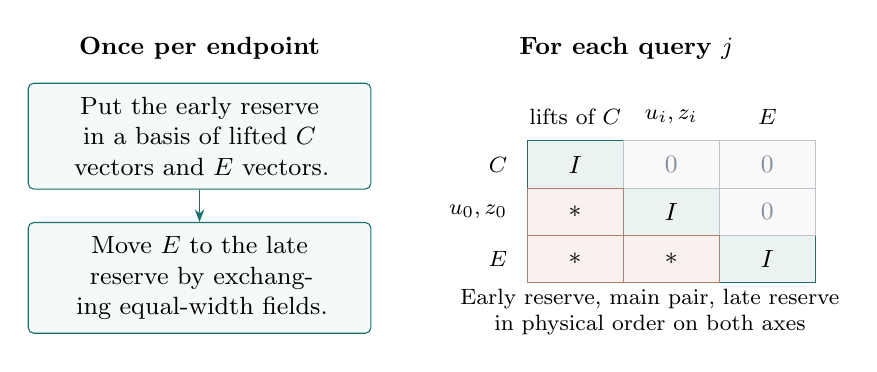
\begin{tikzpicture}[x=1cm,y=1cm,font=\small,
 stage/.style={draw=sea,fill=sea!4,rounded corners=2pt,
  text width=4.0cm,align=center,inner sep=5pt},
 head/.style={font=\footnotesize,align=center},
 block/.style={minimum width=1.22cm,minimum height=.60cm,inner sep=1pt,
   draw=ink!30,font=\small},
 idblock/.style={block,draw=sea,fill=sea!9},
 depblock/.style={block,draw=rust!75,fill=rust!8},
 zeroblock/.style={block,fill=black!2,text=ink!55}]
\node[font=\small\bfseries] at (-3.37,1.72) {Once per endpoint};
\node[stage] (lift) at (-3.37,.60)
  {Put the early reserve in a basis of lifted $C$ vectors and $E$ vectors.};
\node[stage] (late) at (-3.37,-1.20)
  {Move $E$ to the late reserve by exchanging equal-width fields.};
\draw[-{Stealth[length=1.6mm]},draw=sea] (lift)--(late);

\node[font=\small\bfseries] at (2.05,1.72) {For each query $j$};
\node[head] at (1.40,.85) {lifts of $C$};
\node[head] at (2.62,.85) {$u_i,z_i$};
\node[head] at (3.84,.85) {$E$};
\node[head,anchor=east] at (.66,.24) {$C$};
\node[head,anchor=east] at (.66,-.36) {$u_0,z_0$};
\node[head,anchor=east] at (.66,-.96) {$E$};
\foreach \x/\y in {1.40/.24,2.62/-.36,3.84/-.96}
  \node[idblock] at (\x,\y) {$I$};
\foreach \x/\y in {2.62/.24,3.84/.24,3.84/-.36}
  \node[zeroblock] at (\x,\y) {$0$};
\foreach \x/\y in {1.40/-.36,1.40/-.96,2.62/-.96}
  \node[depblock] at (\x,\y) {$*$};
\node[head] at (2.35,-1.63) {Early reserve, main pair, late reserve\\in physical order on both axes};
\end{tikzpicture}
\caption{The address change at one endpoint of a directed rectangle.
The left-hand preparation is shared by all queries. On the right,
columns are the prepared endpoint coordinates, and rows are their
coordinates in the common rectangle layout. Each possible
off-diagonal block ($*$) adds a contribution from an earlier field
to a later one, so the remaining change and its inverse require only
linear-time tape scans. Unshown fields retain their positions during
this per-query change.}
\label{fig:rectangle-layout}
\end{figure}



\paragraph{Delivery by rectangles.}
Write a directed rectangle as $(L,K)$, with sources $L$ and
destinations $K$. To implement $M=I$, evaluate
\eqref{eq:interchange-label-map} on $P_*$ and subtract its value on
each off-diagonal rectangle. For a given rectangle the quantity to
send to every $w\in K$ at a common address $z$ is the same vector
\[
             X_{L,j}(z)=\sum_{v\in L} X_v(S_{v,j}^{-1}z).
\]
Prepare the endpoint changes on the reserved fields once for every
incidence, using copies at the sources. For each $j$ the lower
triangular operations then put the summands of $X_{L,j}$ in the same
physical order. Add them in a scan, retain a copy of their sum, and
send its negative to the destinations of the rectangle. Apply $A_j$
pointwise, and at each destination accumulate the resulting terms
over $j$ after the inverse lower triangular operations. Undo the
change on the reserved fields only after this accumulation.


\paragraph{Delivery at low rank.}
For the $P_*$ contribution choose $r_*$ independent rows $I$ and
$r_*$ independent columns $J$. Over $\mathbb F_p$ we have
\[
              P_*=(P_*)_{:J}\,((P_*)_{IJ})^{-1}\,(P_*)_{I:}.
\]
This factorization uses only $r_*$ intermediate vectors at each
common address. Gathering them directly in one fixed address order
would require reordering all the source streams for each $j$ before
the first matrix could act. Instead, for basis row $i\in I$ the
vector required by $(P_*)_{I:}$ at $z$ is
\[
          X_i(S_{i,j}^{-1}z)+
            \sum_{(L,K):\,i\in K}X_{L,j}(z).
\]
The singleton uses the source layout at $i$. Every other term is a
rectangle sum already produced in its rectangle layout. Disjointness
of the rectangles accounts for each source in the row support exactly
once. There are at most $1+\lambda$ terms, irrespective of the number
of sources in the support. Convert these terms to one fixed layout
for $z$, then add. Each conversion acts on the early and late fields
and $H_j,N_j$, hence costs $O(D)$ calls per internal row. In the
fixed layout apply $((P_*)_{IJ})^{-1}$ and $A_j$ pointwise.

The support of each column in $J$ has the same decomposition on the
destination side. Convert the corresponding intermediate vector to
its singleton layout and to each incident rectangle layout, then
distribute it by the destination lower triangular operations. These
rectangle contributions enter the same destination sums before the endpoint
changes are undone. Finally add together all destined rectangle
contributions and direct singleton contributions at each destination
in its ordinary layout (along with the $A_0$ term).

Thus the changes on reserved fields cost
$O(RND(1+\lambda))$ calls for the entire stage. For each $j$ the
$r_*$ basis rows and $r_*$ basis columns use at most
$2Rr_*(1+\lambda)$ single-stream conversions. They cost
$O(mRr_*D(1+\lambda))$ calls in total, proving
\eqref{eq:interchange-stage-cost}. The row matrices are fixed. Their applications use a finite number of tapes and table entries.


The first term in the call count prepares the endpoints once for
all $m$ queries. The second is the only term that pays a fresh
coordinate change for each query. It does so on the $r_*$ intermediate
streams at each internal row index. Since $m r_*/N$ stays bounded,
these two costs are of the same order after averaging over input
streams.

\subsection{Spectral conversion and the choice of constants}
\label{subsec:swap-spectrum}

Over odd characteristic the swaps $Q_j$ have a common spectral
coordinate system. On each two-element orbit of $Q_j$ place the sum
at the address with $H_j<N_j$ and the difference (smaller address
minus larger address) at the address with $H_j>N_j$. Leave equal
pairs as they are. Apply these changes independently over all $j$.
Each conversion in either direction requires one copied interchange
per pair and pointwise operations, using $1/2$ in the inverse. The
sum and difference coordinates have eigenvalues $1$ and $-1$,
respectively. Since each positive-width field has at least two values,
one may take a two-element orbit in every pair and independently
choose its sum or difference. Thus all $2^m$ sign patterns occur.
To generate the comparisons in linear time,
fix a prefix ending immediately before $N_j$. Its $H_j$ is known,
and its $N_j$-and-suffix fibre splits into three consecutive runs.
If the suffix range is $S$, computing the run lengths takes
$\operatorname{poly}(1+f+\log S)$ steps per prefix, absorbed by the
$b^f S$ positions in the fibre. The elementary-streams lemma provides
the nested scans and amortized counters. An arbitrarily long prefix
index needs only to be advanced, while its controlled field $H_j$
uses $O(f)$ digits.


To compute the whole product $\prod_j Q_j$, use the simultaneous repair
program of \cite[Theorem~\ext{F}{thm:repair} and
Corollary~\ext{F}{cor:swap-repair}]{oaF}. It specifies the batch width
$R$ and a fixed finite scalar extension over $\mathbb F_p$, whose
elements serve as the data alphabet throughout the recursion. At
each common frequency a swap has eigenvalue $+1$ or $-1$. The
program predicts the product of these signs on most of the batch and
recovers the exceptional rows by interpolation. Its table needs only
the sign pattern, which the scans just described generate. The result
on every one of the $R$ independent input streams is exact.

The program uses $O(\sqrt{m\log m})$ stages of
\eqref{eq:interchange-pencil}, pointwise operations, and at most $4s$
full row conversions at each label, where $s\le R/(2m^3)$. Each full
conversion uses $m$ calls. The correction thus costs at most $4ms/R$
calls per input stream. The time spent in the stages is controlled by
\eqref{eq:interchange-stage-cost}.

Choose $1/2<\gamma<\alpha$. Take $q$ to be the smallest power of two
at least $m^{1/p^2}$. Then $m r_*/N=O_p(1)$,
$D=O_p(m^{(2p-1)/p^2})$, and
\[
       D(1+\lambda)\le m^{(3p-1)/p^2+o_p(1)}
          \qquad (m\longrightarrow\infty).
\]
Choose $p$ sufficiently large that $1/2+(3p-1)/p^2<\gamma$.
For sufficiently large fixed $m$, the complete computation of the
main swaps on $W=RN$ independent streams uses at most $Wm^\gamma$
calls. This follows by multiplying \eqref{eq:interchange-stage-cost}
by the number of stages and adding $4ms/R$ per stream for repair.
Also choose $m$ so that
\begin{equation}\label{eq:interchange-contraction}
                         2m^\gamma+2a<m^\alpha .
\end{equation}
All matrices, bases, row widths, and endpoint instructions have now
been fixed. Choose a compatible radix prime $b>W$, with $W>2$.
All linear operations on data, including scalar extension arithmetic,
are fixed finite tables. Recursive calls move symbols of this very
same alphabet, regardless of the depth of recursion.


\subsection{Running the recursion}
\begin{proof}[Proof of Theorem~\ref{thm:interchange}]
First consider two width-$e$ fields in radix $b$, with arbitrary
spectator ranges. Set $f=\lfloor(e-1)/(m+2a)\rfloor$. If $f=0$ the
width is bounded, and individual digit moves cost linear time. For
$f\ge1$, partition each width-$e$ field, from the front, into one
digit, $a$ fields of width $f$, the $m$ main fields of width $f$,
another $a$ fields of width $f$, and a remainder of fewer than $m+2a$
digits. The first group of $a$ fields in the earlier chunk supplies
the early reserve. The second group of $a$ fields in the later chunk
supplies the late reserve.

Split on the first digit of the earlier chunk. Group its $b$ values
into batches of $W$, padding the last batch, and retain the batch
number as a spectator. The result consists of $W$ aligned streams,
each of volume $V'\lceil b/W\rceil/b\le2V'/W$, where $V'$ is the
volume at this recursion node. Splitting, padding, and subsequent
merging cost $O_\alpha(V')$ independently of the prefix range.
Run the finite main-swap computation, implementing each call by this
same general interchange algorithm on a single stream. The complete
operation applies the main swaps to each row separately and preserves
every other address, including both occupied reserves. Discard the
padding and merge. It remains to interchange $2a$ corresponding
pairs of width-$f$ fields and boundedly many pairs of individual
digits. Perform the former recursively on the full stream and the
latter directly.

Let $T(e)$ bound time per symbol of the input stream, uniformly over
the three spectator ranges. The construction gives
\[
            T(e)\le C_\alpha+(2m^\gamma+2a)T(f).
\]
Indeed the main computation makes at most $Wm^\gamma$ calls on
streams of relative volume at most $2/W$. The other $2a$ calls
each have relative volume one. Since $f\le e/m$,
\eqref{eq:interchange-contraction} and induction give
$T(e)=O_\alpha(e^\alpha)$.

For the tape implementation use the depth-first parking schedule of
\cite[Proposition~11]{Tape}. A main call
parks the node's other live streams on stack tapes at their current
ends. Returning to the node restores them from those ends. Clearing
work areas, moving heads, and copying parked streams cost $O_\alpha(V')$
at the node, including all its finitely many descents. The child
descriptor collapses the spectator ranges to the prefix, gap, and
suffix of its two fields. Its calculation and the local control stack
use polynomial time in $1+\log V'$, absorbed by $O_\alpha(V')$.
Space at an active node is $O_\alpha(V')$. A main descent shrinks
volume by a factor at most $2/W<1$. During each of the $2a$
full-volume descents the main streams have already been merged and
their workspace cleared. Pass the active stream to the child and
park only a descriptor and return instruction. Consequently the
parked arrays sum geometrically along any path. The depth is
$O(1+\log(e+1))$ and the parked descriptors have total size
$O_\alpha((1+\log(e+1))(1+\log V'))$ at a root of volume $V'$,
which is $O_\alpha(V')$. Work tapes and their stack areas are reused,
so these bounds also count visited cells.

Finally, for binary chunks take the least $e$ with $b^e\ge 2^u$.
Pad each of the two numerical ranges from $2^u$ to $b^e$ by lexicographic
scans as in \cite[Lemma~12]{Tape}. The volume
increases by a factor less than $b^2$, and the full swap preserves
the set of genuine addresses. Scanning out those addresses returns
the required stream. This costs linear additional time and space,
and $e=O(u)$. Bits are represented by the distinct elements $0,1$ of
the data algebra. A fixed larger input alphabet can be encoded in a
fixed number of bit streams. This proves the theorem.
\end{proof}

\section{Permuting binary addresses on tapes}\label{sec:permutations}

Consider a stream of records with two binary address fields $X,Y$.
One step of the Walsh algorithm sends the record at $(X,Y)$ to
$(X,Y\oplus X)$, where $\oplus$ denotes bitwise addition modulo two.
For three-bit fields, for instance, the record at $(101,011)$ goes to
$(101,110)$. Rotating $Y$ by five modulo eight
gives $000$ in the target field because of the carry. Separately flipping every
bit of $Y$ would require a scan for each bit. We group bit flips into
a small number of shifts and repair the records on which a carry
crosses between groups. This gives a cost governed by the width of
the two fields, which decreases at each level of the Walsh recursion.

Later, the conversion to Chinese remainder coordinates permutes small
blocks of address bits according to other bits of the address. In that
application the available budget depends on the width of the whole
address. We derive both bounds from Theorem~\ref{thm:interchange} and
the bit packing of \cite[Section~5.2]{Tape}.

Fix $1/2<\rho<1$. A stream of $M$ records, each of $R$ bits, has bit
volume $V=MR$. Let $k\ge2$ bound the address width up to a constant
factor, and assume $R=\Theta(k)$ with fixed constants. Scanning the
address counters once per record thus costs $O(V)$. All shapes have
complete ranges in the binary fields on which we operate. A leading
row range can have arbitrary positive integer length, and the spectator
ranges between active fields may be combined. An address permutation
moves whole records and requires no information about their contents.

The elementary stream operations of \cite[Lemma~3]{Tape} move a
single address bit to any position, or permute the four values of any
two specified bits, in $O(V)$ steps. The bounds include the binary
counters, rewinds and cleanup. Descriptors of the fields are supplied
in binary. Throughout this section, the tape count and alphabet are
fixed, the constants in the block widths and polynomial preparation
costs are fixed, and the time bounds include this preparation in the
top parameter $k$ even when the active fields are short. The space
bound in each case is $O(V)+k^{O(1)}$ visited cells. Interchanges
take linear space, and a fixed number of streams suffices for the
scans and sorts below. Adding an $O(k)$-bit address to a record
increases its size by a constant factor.

\subsection{Parallel flips in two address fields}

\begin{lemma}[Bulk XOR between address chunks]\label{lem:packed-xor}
Let $X,Y,Z$ be disjoint complete binary chunks of a common width
$L=O(k)$, occurring in any order with arbitrary intervening spectator
fields. For each target $j$ in a specified set of positions in $Y$,
choose a source position $i(j)$ in $X$. The simultaneous changes
\[
                 Y_j\longleftarrow Y_j\oplus X_{i(j)}
\]
take $O\bigl(V(1+L^\rho)(1+\log k)\bigr)+k^{O(1)}$ fixed multitape
steps. Every other address bit, including all of $Z$, is restored.
\end{lemma}

\begin{proof}
Choose a guard length $G-1$, with $G=C\lceil\log_2(2k)\rceil$ and a
fixed integer $C$ to be chosen below. For one pass, select disjoint
segments of $G$ consecutive bits in $Y$ and the corresponding segments
in $Z$. Write $j$ for the low position of a segment, numbering from bit
zero. We will flip $Y_j$ according to a Boolean control $c_j$ and
restore all other bits of both segments. For this pass we may use
any unchanged controls preceding both chunks, provided the functions
$c_j$ can be computed in $k^{O(1)}$ steps from descriptions of size
$k^{O(1)}$. For $c_j=X_{i(j)}$, interchange equal-width chunks to put
$X$ first and undo the change of layout at the end.

\emph{A shift acting on several segments.}
For two unrestricted integer coordinates $u,w$, let $[u]_h$ indicate
$u\equiv h\bmod2$. The following eight shifts use the current coordinate
values in each assignment, in row order from left to right
\cite[Lemma~13, Equations~(20)--(21)]{Tape}.
\[
\begin{array}{ll}
 u\leftarrow u-c[w]_0 & w\leftarrow w-c[u]_0\\
 u\leftarrow u+c[w]_0 & w\leftarrow w+c[u]_0\\
 w\leftarrow w+c[u]_1 & u\leftarrow u+c[w]_1\\
 w\leftarrow w-c[u]_1 & u\leftarrow u-c[w]_1 .
\end{array}
\]
For $c=0$ these shifts fix both integers. For $c=1$, on each
translated square $\{2a,2a+1\}\times\{2b,2b+1\}$ the first four
assignments cycle the low-bit pairs $(00\ 01\ 10)$ and the last four
cycle $(01\ 10\ 11)$. Their composition flips the low bit of $u$
and restores $w$.

Apply the shifts at all selected segments of $Y,Z$ at once. For
example, one assignment with target $Y$ is the single rotation
\[
      Y\longleftarrow
          Y\mathbin\pm\sum_j2^j c_j[Z_j=h]\pmod{2^L}.
\]
Interchange $Y$ and $Z$ if necessary to place the target last among
these chunks. For every prefix preceding the target, compute the shift
amount from the control bits and the parity bits of the other chunk.
The $2^L$ target values occur consecutively as blocks with a common
suffix length. Split the run at the wrap point and concatenate its two
pieces in rotated order \cite[Lemma~4]{Tape}, keeping each suffix
block intact. Undo the interchange. Each prefix accounts for at least
$2^L\ge2^G$ records whenever there is a segment. Choosing $C$
sufficiently large covers the polynomial cost of calculating one offset
per prefix. With a fixed number of field counters and
Theorem~\ref{thm:interchange}, all eight rotations cost
$O(V(1+L^\rho))+k^{O(1)}$ steps.

\emph{Repairing carries.}
The upper $G-1$ bits of each selected segment form its guard.
Declare an address exceptional if any guard in $Y$ or $Z$ has one of
its first ten or last ten values. At every other address the integer
in each segment stays inside its $G$ bits throughout the eight shifts,
since its displacement is at most eight. Thus the performed permutation
$S$ agrees there with the desired controlled flips $D$. The map $D$
preserves every guard. Both $S$ and $D$ are bijections and agree on the
complement of the exceptional set $\mathcal B$, so they both preserve
$\mathcal B$. The remaining permutation $DS^{-1}$ need only be applied
to records now in exceptional slots.

With $s$ segment pairs the exceptional fraction is at most
$80s2^{-G}$, also within any fixed row, since each guard assumes all
$2^{G-1}$ values equally often. A scan identifies these records in
$O(k)$ steps per address using prepared masks for the guards. It
suffices to read their four low bits and test whether the higher bits
are all zero or all one. Extract each exceptional record and attach
its destination rank. Compute this rank from its current address by
reversing the eight rotations and then performing the prescribed bit
flips. This takes $k^{O(1)}$ steps per extracted record, including
address arithmetic in the rectangular layout. Sort these tagged
records by destination with $O(k)$ stable binary radix passes, then
merge them into the exceptional slots in stream order. Beyond setup
and full scans, this costs
\[
             |\mathcal B|\bigl(k^{O(1)}+O(kR)\bigr).
\]
There are $s=O(k)$ segment pairs. After fixing the polynomial bounds
for the controls, offsets and rank calculations, take $C$ large enough
that this cost is $O(V)$. This proves an exact pass even when all
auxiliary address values are occupied.

\emph{Covering the targets.}
Partition the target positions $j$ with $j+G\le L$ by their residues
modulo $G$. Within each class the segments are disjoint, so one pass
with $c_j=X_{i(j)}$ suffices. At most $G-1$ high positions have too
little room for a guard. Treat each by the elementary two-bit operation
on $X_{i(j)},Y_j$. This also handles the entire case $L<G$. There are
$O(1+\log k)$ passes in all.
\end{proof}

\subsection{Permuting positions and blocks}

\begin{corollary}[Permutations of address positions]\label{cor:bit-positions}
An explicitly specified permutation of the $k$ binary address positions
of $2^k$ records takes
$O_\rho(V(1+k)^\rho(1+\log k))$ deterministic fixed multitape steps.
\end{corollary}

\begin{proof}
A permutation is a product of two involutions. On each cycle, number
positions modulo its length and use the reflections $i\mapsto-i$ and
$i\mapsto1-i$ in that order. It suffices to perform the disjoint pairs
of exchanges in one involution. Split the address into three chunks
of width $\lfloor k/3\rfloor$ and at most two remaining bits. Handle
the pairs touching the remaining bits individually. Between any two
chunks perform all exchanges with three simultaneous XORs, using
the third chunk as the auxiliary chunk in Lemma~\ref{lem:packed-xor}.
Within a single chunk, assign a distinct temporary position $t$ in
another chunk to each exchange $(i,j)$. The three cross-chunk exchanges
$(i,t),(j,t),(i,t)$ effect $(i,j)$ and restore $t$. This uses a
bounded number of applications of the lemma. The $k^{O(1)}$ steps to
prepare the cycle decompositions and position lists are absorbed by
the full $2^k$-record volume.
\end{proof}

The Chinese remainder layout in Section~\ref{sec:integers} needs to
rotate the values of each of several short fields by amounts determined
by other address bits. The next lemma allows an arbitrary permutation
table for each such field, including a different table for every
assignment of the controls.

\begin{lemma}[Controlled permutations on small blocks]\label{lem:controlled-blocks}
On a full $k$-bit address space, take pairwise disjoint target blocks of
$O(\log(2k))$ specified bit positions each. Fix $\delta>0$ and a common
set of at most $(1-\delta)k$ control positions disjoint from the targets.
At each block prescribe a permutation of its values depending on the
control bits. At any control setting its table must be generable in
$k^{O(1)}$ tape steps, with uniform polynomial bounds on this computation
and its description. Applying all block permutations, or all their
inverses, to the records takes
\[
 O\bigl(V(1+k)^\rho(1+\log k)^3\bigr)+k^{O(1)}
\]
deterministic fixed multitape steps.
\end{lemma}

\begin{proof}
We first perform controlled flips on a batch of $b$ individual targets,
where $b\le c_\delta k/G$ for a sufficiently small $c_\delta>0$ and
$G$ is the guard parameter above. By Corollary~\ref{cor:bit-positions},
place all controls first and the targets at the low positions of $b$
disjoint $G$-bit segments of a chunk $Y$. Reserve a further $bG$
positions for $Z$. The two chunks fit in the at least $\delta k$ free
positions. Use the guarded pass from Lemma~\ref{lem:packed-xor} and
undo the rearrangement. Including the two position permutations, the
cost of one batch is $O(V(1+k)^\rho(1+\log k))+k^{O(1)}$. Thus a
layer of flips on all targets costs
$O(V(1+k)^\rho(1+\log k)^2)+k^{O(1)}$. Bounded $k$ can always be
handled by a direct split and merge.

For arbitrary block permutations we also need the other bits of each
active block as controls. Batch the blocks so that each batch uses at most
$\delta k/2$ positions and at most $c_{\delta/2}k/G$ blocks.
Greedily filling batches yields $O(1+\log k)$ batches. For large $k$,
a width-limited batch occupies $\Omega_\delta(k)$ positions since the
next block has only $O(\log k)$ bits. A count-limited batch contains
$\Omega_\delta(k/G)$ blocks.

Ignore empty blocks. On a $d$-bit block with $d\ge1$, any permutation of the $2^d$ values is realized by
a Bene\v{s} network with $2d-1$ stages \cite{benes}. Each stage flips
one fixed bit as a function of all other bits. For the construction,
pair inputs differing in one chosen bit, and pair outputs the same way.
The permutation gives a degree-two bipartite multigraph on the input
and output pairs. Alternating colors on each cycle, including a doubled
edge, assign one edge of each color to every pair. An input switch and
an output switch along the chosen bit place the colors in separate
classes. Recurse within each class on the remaining $d-1$ bits, with
one switch when $d=1$. The successive target positions are fixed, and
the switch decisions are computable from the permutation table in time
polynomial in $2^d$. Inverting the tables gives the inverse operation.

Align these schedules within each batch, padding shorter schedules by
identities. At one stage keep all active block bits except the current
targets among the controls. Together with the external controls they
use at most $(1-\delta/2)k$ positions. There is at most one target per
block, so a single batch of guarded flips implements the stage.
Multiplying the cost of that batch by $O(1+\log k)$ stages and
$O(1+\log k)$ block batches gives the bound.
\end{proof}

\section{Normalized Walsh layers on tapes}\label{sec:tape-walsh}

The multiplication algorithm uses short Fourier transforms on several
address fields at once. Their factorization in Section~\ref{sec:integers}
requires a Walsh transform on one selected bit in each of several
fields. On one bit the transform is the normalized butterfly
\[
        (u,v)\longmapsto ((u+v)/\sqrt2,(u-v)/\sqrt2).
\]
Write \(H=2^{-1/2}\bigl(\begin{smallmatrix}1&1\\1&-1\end{smallmatrix}\bigr)\)
for its matrix. Given a set of bits in a \(k\)-bit address, a
\emph{selected-bit Walsh layer} applies \(H\) on those bits and the
identity on the rest. Fixing the other bits gives independent copies
of the same transform. The cost on tapes includes gathering those
copies, performing the transform at fixed precision, and returning
every record to the prescribed order.

\begin{lemma}[Selected-bit Walsh layers]\label{lem:tape-walsh}
Fix \(1/2<\rho<1\) and constants \(c,L,D>0\).
Let \(N=2^k\), \(k\ge1\), and specify
\(s\le ck/\log(2+k)\) distinct address bits. There is a complex
fixed-point format with fractional and signed integer widths equal to
fixed multiples of \(k\) in each real component. The multiples depend
only on \(\rho,c,L,D\). Given \(N\) records in lexicographic order
representing a vector \(x\) with \(\|x\|_2\le2^{Lk}\), a deterministic
fixed multitape machine computes the selected-bit Walsh layer to
absolute Euclidean error at most \(2^{-Dk}\). Its output has the
same format and order. It takes
\[
 O_{\rho,c,L,D}\!\left(Nk(1+k)^\rho(1+\log(2+k))\right)
\]
steps, including address changes and scalar preparation, and visits
\(O_{\rho,c,L,D}(Nk)\) cells. In the exact execution, the maps from the
input to any intermediate numerical array and from an additive error
in such an array to any later numerical array or output have operator
norm at most \(C(1+k)^B\) for fixed \(C,B\). The same bounds hold for
the adjoint layer.
\end{lemma}

\begin{proof}
Use Corollary~\ref{cor:bit-positions} to move the selected positions
to the low \(s\) bits. The other bits now index \(q=2^{k-s}\) spectator
rows, each holding a complete range of \(2^s\) addresses. The empty
selection is the identity. For odd \(s\) apply one butterfly directly
and transform the remaining \(s-1\) bits. Splitting into the two bit
classes aligns the operands for a scan of sums, differences and
scalings, followed by a merge. At the precision chosen below this
takes \(O(Nk\log(2+k))\) steps, including head returns. Bisection
with dyadic integer-square comparisons prepares \(1/\sqrt2\) to that
precision in \(k^{O(1)}\) steps. This settles \(s=1\). In every case
undo the initial bit-position permutation after the arithmetic.

\paragraph{A batch of transforms.}
Use the normalized binary construction in
\cite[Proposition~\ext{F}{prop:binary-template}, Equation~(\ext{F}{eq:kernel-template-saving})
and Section~\ext{F}{sec:prime-kernel}]{oaF}. It supplies fixed integers
\(A\ge3\), \(W\) and \(\sigma\). On \(W\) rows with \(Af\) address
bits per row, it implements a normalized transform of those bits by
\(\sigma\) child calls, each transforming one \(f\)-bit slot of one
work row on all its fibers. Here \(f\) is even. The strict saving is
\[
                            \sigma/W<A^\rho .
\]
We may duplicate the batch and all its calls to obtain \(W\ge2\).
Apart from the calls, the finite instruction list combines aligned
rows and changes their addresses. Pointwise scalar choices depend on
parities of sums of fixed functions of the \(f\) columns, each an
\(A\)-bit tuple with one bit from each slot. An address change applies
a fixed invertible binary matrix to every column. The scalars lie
in a fixed finite dyadic list because the normalized child transforms
already supply the normalization factors. The finite construction is
effective for rational \(\rho\). For any other admissible \(\rho\)
one can use a rational exponent strictly between \(1/2\) and \(\rho\).

Divide the even part of the selected width into pieces sized for this
recursion. Write \(\lfloor s/2\rfloor=\sum_{j=0}^J b_jA^j\), with
\(0\le b_j<A\). Allocate \(b_j\) consecutive pieces of width \(2A^j\)
and transform the pieces in succession. Append zero spectator rows to
make \(q'\), the padded leading row count, a multiple of \(W^J\).
Since \(W^J\le(1+s)^{O_\rho(1)}\) and \(q\ge2^{k/2}\) for large \(k\),
we have \(q'\le2q\). The bounded remaining widths admit direct
butterflies. Each full piece transform acts independently on all
spectator coordinates, so the added rows may be removed after the
last piece.

\paragraph{A recursive call on tapes.}
At a node with \(a=2A^j\) consecutive active bits, \(j>0\), the
leading row count \(r\) is divisible by \(W^j\). Set \(f=a/A\).
Split the leading rows by their residues modulo \(W\) onto \(W\)
streams. The entries at the same position on these streams supply the
aligned operands for one batch operation. Each stream has exactly
\(1/W\) of the parent's volume and leading count \(r/W\), divisible
by \(W^{j-1}\). Each child takes one work stream, designates one of
its \(f\)-bit slots as active, and leaves every other field as a full
spectator range. Figure~\ref{fig:walsh} shows this repeated layout.
The outputs merge by reversing the split. At \(a=2\) use the
four-point Walsh transform with coefficients \(\pm1/2\), splitting
and merging its four bit classes in a bounded number of scans.

\begin{figure}[!htb]
\centering
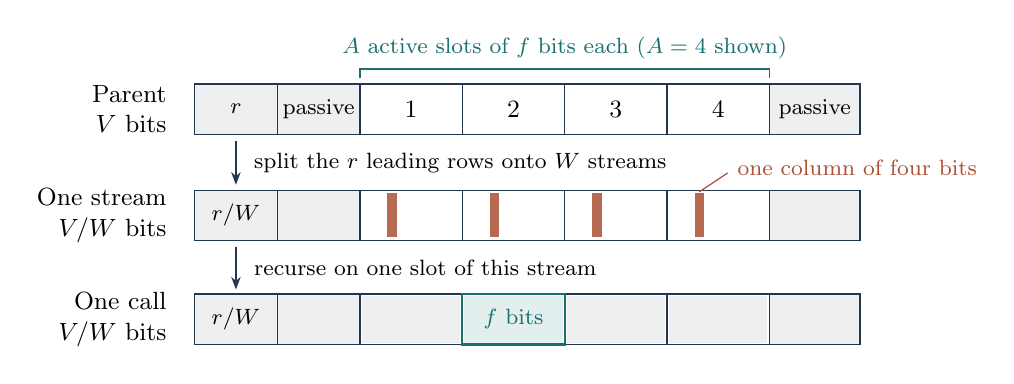
\begin{tikzpicture}[font=\small, x=1cm, y=1cm, line width=.52pt,
   descriptor/.style={anchor=east,align=right,font=\small},
   arrow/.style={draw=ink,-{Stealth[length=1.6mm]}}]
% Horizontal positions denote address fields, not their numeric widths.
\newcommand{\slotrow}[3]{%
  \fill[ink!8] (0,#1) rectangle (2.1,#1+.64);
  \fill[ink!8] (7.3,#1) rectangle (8.45,#1+.64);
  \draw[ink] (0,#1) rectangle (8.45,#1+.64);
  \foreach \cut in {1.05,2.1,3.4,4.7,6,7.3}
     \draw[ink] (\cut,#1)--(\cut,#1+.64);
  \node[font=\footnotesize] at (.525,#1+.32) {#2};
  \node[descriptor] at (-.23,#1+.32) {#3};}
\slotrow{2.35}{\(r\)}{Parent\\\(V\) bits}
\node[font=\footnotesize] at (1.575,2.67) {passive};
\node[font=\footnotesize] at (7.875,2.67) {passive};
\foreach \x/\txt in {2.75/1,4.05/2,5.35/3,6.65/4}
  \node at (\x,2.67) {\(\txt\)};
\draw[sea] (2.1,3.06)--(2.1,3.18)--(7.3,3.18)--(7.3,3.06);
\node[text=sea,above,font=\footnotesize] at (4.7,3.18)
  {\(A\) active slots of \(f\) bits each (\(A=4\) shown)};

\draw[arrow] (.525,2.26)--(.525,1.71)
  node[midway,right,font=\footnotesize,xshift=3pt]
  {split the \(r\) leading rows onto \(W\) streams};
\slotrow{1}{\(r/W\)}{One stream\\\(V/W\) bits}
\foreach \x in {2.45,3.75,5.05,6.35}
  \fill[rust!85] (\x,1.04) rectangle (\x+.12,1.60);
\node[font=\footnotesize,text=rust,anchor=west] at (6.77,1.92)
  {one column of four bits};
\draw[rust,line width=.45pt] (6.77,1.86)--(6.41,1.62);

\draw[arrow] (.525,.92)--(.525,.38)
  node[midway,right,font=\footnotesize,xshift=3pt]
  {recurse on one slot of this stream};
\slotrow{-.32}{\(r/W\)}{One call\\\(V/W\) bits}
\foreach \x in {2.1,4.7,6}
   \fill[ink!8] (\x+.025,-.30) rectangle (\x+1.275,.30);
\fill[sea!12] (3.425,-.30) rectangle (4.675,.30);
\draw[sea,line width=.8pt] (3.4,-.32) rectangle (4.7,.32);
\node[font=\footnotesize,text=sea] at (4.05,0) {\(f\) bits};
\end{tikzpicture}
\caption{One level of the Walsh recursion. The leading range counts
rows. The orange marks pick the same offset in each slot, so a
column change acts across slots. Each child transforms one whole slot
on every setting of its spectator fields. Other work streams remain
parked until the child returns.}
\label{fig:walsh}
\end{figure}


Let \(V\) be the bit volume of the node, including spectator ranges
and record widths. Binary elimination factors a column change into
a fixed number of slot exchanges and slot additions. An exchange uses
Theorem~\ref{thm:interchange}. For an addition, apply
Lemma~\ref{lem:packed-xor} with source and target slots of width \(f\)
and a third slot as auxiliary. All three ranges are complete, the
auxiliary contents are restored, and the leading range \(r/W\) may
have arbitrary length. These address changes together take
\[
 O_\rho\!\left(V(1+a^\rho)(1+\log(2+k))\right)+k^{O_\rho(1)}
\]
steps, including the narrow slots handled by direct bit operations
in Lemma~\ref{lem:packed-xor}. Pointwise passes take
\(O_\rho(V\log(2+k))+k^{O_\rho(1)}\) steps. To select a scalar, copy
the slots from the address counter onto separate tapes, scan all the
columns in parallel, accumulate the required parities, and rewind.
Even a scan of the full \(O(k)\)-bit address per record is paid for
by its width \(\Theta(k)\). There are only finitely many operands per
pointwise operation. Fixed dyadic scalings use short exact products
before rounding. A general product of two \(O(k)\)-bit numbers, as
in the direct butterfly, costs \(O(k\log(2+k))\) tape steps \cite{hvh}.

\paragraph{Work and visited space.}
Follow the depth-first schedule of \cite[Proposition~11]{Tape}.
Park the other streams and the parent descriptor on end-access stacks
while one child runs. On return, restore them to their marked work
areas. Copying, parking, erasing and rewinding add
\(O_\rho(V)+k^{O_\rho(1)}\) work per node. The child needs access only
to its current work areas and descriptors. Row counts, active widths,
and prefix, gap and suffix lengths fit in \(O_\rho(k)\)-bit descriptors
and all fixed-arity descriptor computations take \(k^{O_\rho(1)}\)
steps.

With the record width fixed throughout, divide time by volume and
write \(T(a)\) for the resulting bound at active width \(a\), omitting
the additive polynomial setup costs. The \(V/W\) volume of each child
gives
\[
 T(a)\le C_\rho(1+a^\rho)(1+\log(2+k))
                 +(\sigma/W)T(a/A).
\]
Relative to \(a^\rho\), successive levels have ratio
\(\sigma/(WA^\rho)<1\). Geometric summation with the four-point base
case yields \(T(a)=O_\rho(a^\rho(1+\log(2+k)))\). Also
\(\sum_j b_j(2A^j)^\rho=O_\rho(s^\rho)\). Each piece has constant
branching and depth \(O(\log(2+k))\), so all polynomial setup terms
together remain \(k^{O_\rho(1)}\), absorbed by \(N=2^k\). Including
both position permutations and the one-bit butterfly gives the
claimed time on a padded volume of \(O(Nk)\).

One node needs a fixed number of \(O(V)\)-bit streams for its scans
and for the sparse repair sort in Lemma~\ref{lem:packed-xor}.
Theorem~\ref{thm:interchange} also uses linear space. Along a single
descent, the parked volumes are bounded by a constant multiple of
\(V+V/W+V/W^2+\cdots\). Siblings and successive pieces reuse the
same tape regions. The additional descriptor and word workspace
along the stack is \(k^{O_\rho(1)}\), so the total number of visited
cells is \(O_{\rho,c,L,D}(Nk)\).

\paragraph{Precision.}
Give each concatenated set of live numerical arrays its Euclidean
norm. At one node there are a bounded number of operations on the
live arrays. Each has bounded norm when a completed child is counted
as one operation, since its transform on all fibers is unitary.
Copies and pointwise combinations have bounded norm from their
fixed coefficient and stream lists, and permutations are isometries.
For an input-to-intermediate estimate, descend only into the successive
calls containing the given array. An error originating inside a child
can propagate through its returned stream to the first common ancestor
of its operation and a later one, then down to the later array. At
most a constant norm factor is incurred per visited level. The depth
is logarithmic in \(k\), giving polynomial gain. If the two operations
occur in different pieces, all complete intervening pieces are
unitary on the padded array. Padding and restriction themselves have
norm at most one.

Round each real component after arithmetic to a grid of mesh \(2^{-p}\).
Choose \(1/\sqrt2\) to absolute error at most \(2^{-p}\) and store the
fixed dyadic coefficients exactly. Temporarily allow unbounded integer
parts. Rounding an array costs at most a constant times
\(\sqrt N\,2^{-p}\) in Euclidean norm. The approximate butterfly
coefficient introduces an additional error of at most a constant times
\(2^{-p}\) times the input norm. Thus while all preceding array norms
are at most \(2^{(L+2)k}\), a single operation incurs at most
\[
 C_\rho\,2^{-p}\bigl(\sqrt N+2^{(L+2)k}\bigr).
\]
Each array contains at most a fixed multiple of \(N\) entries. There
are \(k^{O_\rho(1)}\) array operations. Freeze their actual rounding
faults and propagate these vectors through the exact linear maps.
The polynomial gain bound then shows that \(p=\lceil C_{\rho,c,L,D}k\rceil\)
makes the total error at any array at most \(2^{-Dk}\), for a
sufficiently large constant. The corresponding ideal intermediate
norms are at most \(C(1+k)^B2^{Lk}\). For large \(k\) induction
therefore preserves the assumed norm bound, justifying signed integer
width \(O_{\rho,c,L,D}(k)\). Temporary exact sums and products before
rounding have the same order of width. Enlargement of the constant
width factors covers the bounded remaining lengths. Finally, the layer
is self-adjoint since \(H=H^*\).
\end{proof}

\section{Integer multiplication on fixed tapes}\label{sec:integers}

Write each input as a polynomial evaluated at a power of two. To
multiply the integers it suffices to convolve the coefficient lists
exactly and propagate carries. We compute this convolution with two
forward Fourier transforms, one coordinatewise product and one
inverse transform. On tapes, the choice of the transform length
determines how much time is spent reaching the records that each
operation needs.

\begin{theorem}[Multiplication at a fixed exponent]\label{thm:integer}
For each \(\epsilon>0\) there is a deterministic multitape Turing
machine, with fixed alphabet and tape count, that computes the full
product of two \(n\)-bit integers in worst-case time
\(O_\epsilon(n(1+\log n)^{1/2+\epsilon})\), visiting
\(O_\epsilon(n)\) cells on its tapes.
\end{theorem}

Fix \(\epsilon>0\), and choose a rational exponent
\(\tfrac12<\rho<\min\{1,\tfrac12+\epsilon\}\) for
Theorem~\ref{thm:interchange} and Lemma~\ref{lem:tape-walsh}.
We will store the digits in \(N=2^k\) records of width \(O_\rho(k)\),
with \(k=\Theta(\log n)\) and \(Nk=\Theta(n)\). We arrange the
convolution on many short cyclic axes. Each transform then needs
only \(O(\log k)\) layers of record permutations, phase
multiplications and selected-bit Walsh transforms, preserving
the Euclidean norm at every layer boundary. The time budget for
Theorem~\ref{thm:integer} is
\begin{equation}\label{eq:integer-budget}
 O_\rho\!\left(Nk(1+k)^\rho(1+\log(2+k))^{O(1)}\right).
\end{equation}
Products within a single record of \(O(k)\) bits take
\(O(k\log(2+k))\) steps with the multitape multiplier of
Harvey and van der Hoeven \cite{hvh}. Marking the extents of its
scratch areas lets us clear them and return the heads within the
same time bound.

\subsection{Packing the digits into short cyclic axes}

For \(n=1\) use direct multiplication. For \(n\ge2\), let
\(X(t)=\sum_{u<h}x_u t^u\) and \(Y(t)=\sum_{u<h}y_u t^u\)
be the radix-\(2^b\) expansions of the inputs, with
\(0\le x_u,y_u<2^b\). Set
\[
 b=\lceil\log_2 n\rceil,\qquad h=\lceil n/b\rceil,\qquad
 k=\lceil\log_2(4h)\rceil,\qquad N=2^k.
\]
A cyclic convolution of length at least \(2h-1\) recovers every
coefficient of \(X(t)Y(t)\). We choose its length \(S\) as a product
of pairwise coprime factors \(a_i\). Factor \(a_i\) has an address
field of \(l_i\) bits, so its padded axis has \(2^{l_i}\) positions.
We require
\begin{equation}\label{eq:integer-box}
 \sum_i l_i=k,\qquad \max_i l_i=O(\log k),\qquad
 d=O(k/\log k),\qquad S:=\prod_{i=1}^d a_i\ge 2h .
\end{equation}
Short axes give polynomial-size tables in \(k\). Filling a constant
fraction of the padded box ensures that these tables can act on a
stream of only \(O(h)\) records, even with separate binary address
fields for all \(d\) axes.

For all sufficiently large \(k\), put \(l=20\lceil\log_2 k\rceil\)
and \(x=2^l\). Take \(\lfloor k/l\rfloor\) distinct odd primes
from \([x(1-k^{-2}),x]\), each with \(l_i=l\). If \(l\) does not
divide \(k\), append \(a_d=2^{k\bmod l}\), with \(l_d=k\bmod l\).
Baker, Harman and Pintz \cite{bhp} give a prime in
\([y-y^{0.6},y]\) for all sufficiently large \(y\). The chosen
interval contains \(k\) disjoint intervals of this form with right
endpoints near \(x\), since \(kx^{0.6}=o(x/k^2)\). Enumeration
and trial division take \(\operatorname{poly}(k)\) bit steps because
\(x=k^{O(1)}\). The resulting volume satisfies
\[
 S\ge N(1-k^{-2})^{\lfloor k/l\rfloor}\ge N/2\ge 2h.
\]
The machine tests the size and coprimality conditions and uses
direct multiplication on the bounded initial range where they fail.

Store the \(N\) positions in lexicographic order on the padded
axes \(d,d-1,\ldots,1\), with axis \(1\) varying fastest. A valid
address has digits \(t_i<a_i\) for every \(i\). In tape order, these
valid addresses enumerate the ranks \(0,\ldots,S-1\) in mixed radix.
Count the input length with an amortized binary counter and reverse
the streams to read their low bits first. As the machine enumerates
the box it places the successive radix-\(2^b\) digits at the first
\(h\) valid addresses, writing zero at every other position. A
simultaneous scan of the \(k\) address bits and the marked fields
containing their limits tests validity in \(O(k)\) steps. The writes,
scans and rewinds together cost \(O(Nk)\).

\subsection{Changing from digit order to residue order}

The digits enter the tape in increasing order of their mixed-radix
rank. For convolution the indices must add coordinatewise modulo the
\(a_i\). Put \(P_i=\prod_{j<i}a_j\) and
\(\mu_i=P_i^{-1}\bmod a_i\). If \(t=\sum_iP_it_i\) has digits
\(t_i\), use the scaled residue
\begin{equation}\label{eq:integer-crt}
 y_i=\mu_i t\bmod a_i
     =t_i+\mu_i\sum_{j<i}P_jt_j\bmod a_i .
\end{equation}
These coordinates give an isomorphism
\(\mathbb Z/S\mathbb Z\to\prod_i\mathbb Z/a_i\mathbb Z\).
The scaling by \(\mu_i\) makes the coefficient of the current digit
one. The permutation can therefore use rotations controlled by
earlier digits, as in the prime-factor algorithm \cite{good} and the
triangular layout of \cite[Equation~(42)]{Tape}.

Build a balanced binary tree of consecutive axis intervals, splitting
an interval after the first \(\lfloor |I|/2\rfloor\) axes. The map for
\(I\) is Equation~\eqref{eq:integer-crt} with the sum restricted to
\(j\in I\). A leaf is the identity. Once the two child maps have been
applied, each right-child axis \(i\) only needs the rotation
\[
       \mu_i\sum_{j\ \mathrm{in\ the\ left\ child}} P_jt_j
       \pmod {a_i}.
\]
The current left-child address determines its original digits \(t_j\)
by solving the triangular equations in increasing order. Use zero
rotation for an invalid left-child address and fix values outside
\([0,a_i)\) on each target axis. Each step is then a permutation of
the full padded box. For the inverse map, reverse the depth order
and negate the rotations.

Lemma~\ref{lem:controlled-blocks} combines all disjoint intervals at
one depth as a single controlled permutation. The control
bits lie in the left children, which collectively contain at most
half the axes. Since all fields except possibly the last have equal
width, the controls occupy at most \(k/2+O(\log k)\) bits. The target
blocks have width \(O(\log k)\). For a given control setting we can
recover the left digits and generate all local rotation tables in
\(\operatorname{poly}(k)\) steps. The integers \(P_j\) have at most
\(k+1\) bits and a table has at most \(2^l=\operatorname{poly}(k)\)
entries. The lemma charges for generating these tables as well as for
moving the records. A constant fraction of address bits lies outside
the controls, so the lemma applies at every depth. The \(O(\log k)\)
depths fit the budget in Equation~\eqref{eq:integer-budget} in both
directions.

\subsection{Short Fourier transforms on occupied fibers}

After the CRT permutation, each factor has length \(a_i\), but its
address occupies \(l_i\) bits. A radix-two chirp computation may need
several times as many coordinates as fit along that axis. Padding
every axis by such a factor would increase the size of the tensor
product exponentially in the number of axes. Instead we borrow
coordinates from adjacent fibers, perform a short transform, and
restore the borrowed values exactly in the ideal complex arithmetic.

Write \(e(t)=\exp(2\pi i t)\), and put
\[
 U_a=\bigl(a^{-1/2}e(jh/a)\bigr)_{0\le j,h<a},\qquad
 H=2^{-1/2}\begin{pmatrix}1&1\\1&-1\end{pmatrix}.
\]
\begin{lemma}[Synchronized short Fourier transforms]\label{lem:synchronized-short}
For the axis lengths and widths of Equation~\eqref{eq:integer-box},
let \(k\) be sufficiently large. On the \(N=2^k\) coordinates of the
padded residue array, both
\[
             \mathcal U=\bigotimes_i(U_{a_i}\oplus I_{2^{l_i}-a_i})
             \qquad\text{and}\qquad \mathcal U^*
\]
factor into \(O(\log(2+k))\) unitary layers. Partition the axes into
disjoint consecutive blocks of \(O(\log(2+k))\) address bits each.
Every layer has one of the following forms.
\begin{enumerate}
\item A permutation acting independently within each block.
\item A diagonal whose value at an address is the product of one
      unit-modulus coefficient from each block.
\item A normalized Walsh transform on one designated bit from each
      participating block, using \(O(k/\log(2+k))\) bits in total.
\end{enumerate}
For any fixed \(C>0\), a deterministic fixed-tape machine constructs
the schedule, the block permutations, and the block phase tables
at \(Ck+O(\log(2+k))\) fractional bits in \(\operatorname{poly}_C(k)\)
steps. It can then stream the coefficients of any full diagonal to
absolute error \(2^{-Ck}\) in \(O_C(Nk\log(2+k))\) steps.
\end{lemma}

\begin{proof}
It suffices to construct the forward transform. Reversing the schedule,
inverting the permutations and conjugating the phases gives its adjoint.

\paragraph{An exact transform on occupied coordinates.}
Fix an axis of length \(a\), and take the least power of two
\(r\ge 2a-1\). Inside \(\mathbb C^{2r}\) let \(T\) be the space of
the first \(a\) coordinates and \(P\) its orthogonal projection.
We construct \(U_a\oplus I_{2r-a}\) in \(O(\log a)\) layers of
permutations, phase diagonals and operations on disjoint pairs.
The inequality \(2r<8a\) will bound the number of neighboring values
to borrow.

A truncated chirp gives a unitary \(V\) whose compression to \(T\)
is a fixed positive multiple of \(U_a\). In detail, zero-extend
\(a^{-1/2}e(-h^2/(2a))\), \(|h|<a\), to a cyclic kernel of length
\(r\). Its Fourier multipliers are
\[
              \lambda_\xi
        =a^{-1/2}\sum_{|h|<a} e(-h^2/(2a)+\xi h/r).
\]
We show below that \(|\lambda_\xi|\le40\), uniformly in \(a,\xi\).
Choose \(J=64\) and \(\phi=\pi/(4J+2)\). With
\(z=\lambda_\xi\sin\phi\) we have \(|z|\le40\pi/258<1/2\).
Apply \(U_r\) on the first \(r\) coordinates, act on each pair
\((\xi,r+\xi)\) by the unitary
\[
             L(z)=
             \begin{pmatrix}z&\sqrt{1-|z|^2}\\
                            \sqrt{1-|z|^2}&-\overline z\end{pmatrix},
\]
then apply \(U_r^*\) on the first \(r\) coordinates. The compression
to these \(r\) coordinates is convolution by the truncated chirp
times \(\sin\phi\). The differences \(j-h\) of two indices of \(T\)
lie in \((-a,a)\), so their representatives in this interval are
unambiguous modulo \(r\). Multiplying the
active coordinates by \(e(j^2/(2a))\) before and after the
convolution therefore gives Bluestein's factorization
\cite{bluestein}. For the resulting unitary \(V\) we have
\(PV|_T=\sin\phi\,U_a\).

Amplitude amplification now makes the first block exact
\cite{BHMT,berry,MZ}. For each vector \(v\) of an orthonormal basis
of \(T\), put \(w_v=(I-P)Vv/\cos\phi\). These vectors in \(T^\perp\)
are orthonormal because both \(V\) and \(U_a\) are isometries.
In the plane spanned by \(w_v,U_av\),
\[
                    Vv=\cos\phi\,w_v+\sin\phi\,U_av .
\]
The reflection \(I-2P\) fixes \(w_v\) and reverses \(U_av\). On this
plane \(2VPV^*-I\) reflects across \(Vv\), since the other vectors
of the basis of \(V(T)\) are orthogonal to the plane. The product
of the reflections rotates through \(2\phi\) towards \(U_av\).
Consequently
\[
                  B=\bigl[(2VPV^*-I)(I-2P)\bigr]^J V
                    = U_a\oplus B'
\]
for a unitary \(B'\) on \(T^\perp\), since \((2J+1)\phi=\pi/2\).
The only reflection we must implement in the original coordinates
is a diagonal sign change.

To restore the neighboring values, we use \(B\) as a change of basis.
The chirp
\[
             \chi(t)=e\bigl((t^2+(a\bmod 2)t)/(2a)\bigr)
\]
is \(a\)-periodic, and \(\chi(j)\chi(-h)/\chi(j-h)=e(jh/a)\).
Thus \(U_a=D_1 C D_3\), where \(D_1(j)=\chi(j)\), \(D_3(h)=\chi(-h)\)
and \(C\) is the circulant with kernel \(a^{-1/2}\overline{\chi(t)}\).
In the Fourier basis \(D_2=U_aCU_a^*\) is a diagonal of phases,
\[
               D_2(\xi)=a^{-1/2}
                    \sum_{h=0}^{a-1}\overline{\chi(h)}e(\xi h/a).
\]
Extending each of the three diagonals by the identity gives
\[
 (D_1\oplus I)B^*(D_2\oplus I)B(D_3\oplus I)=U_a\oplus I.
\]
Indeed the middle conjugation acts by \(C\) on \(T\) and by
\((B')^*B'=I\) on its complement. The identity holds on arbitrary
data in the borrowed coordinates (Figure~\ref{fig:borrow}).
Each use of \(U_r\) or its adjoint has radix-two depth \(O(\log a)\)
\cite{cooleytukey}, and the number of such uses is absolute.

\begin{figure}[!htbp]
\centering
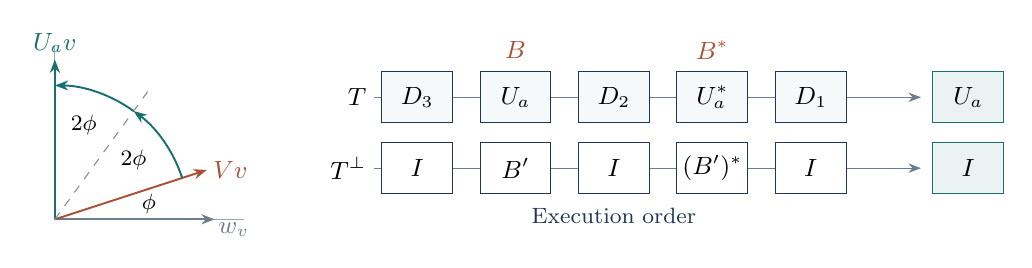
\begin{tikzpicture}[
   font=\small, >=Stealth,
   amp/.style={line width=.7pt,-{Stealth[length=1.7mm]}},
   layer/.style={minimum width=9mm,minimum height=6.5mm,
                 draw=ink,inner sep=1.5pt,fill=white,font=\small},
   result/.style={layer,fill=sea!9,draw=sea}
]
\begin{scope}
 \draw[ink!45] (2.4,0)--(0,0)--(0,2.2);
 \draw[amp,ink!65] (0,0)--(2.03,0)
       node[below right,inner sep=1pt] {$w_v$};
 \draw[amp,sea] (0,0)--(0,2.03) node[above,inner sep=2pt] {$U_av$};
 \draw[amp,rust] (0,0)--(18:2.03) node[right,inner sep=2pt] {$Vv$};
 \draw[ink!55,dashed] (0,0)--(54:2.03);
 \draw[sea,amp] (18:1.7) arc[start angle=18,end angle=54,radius=1.7];
 \draw[sea,amp] (54:1.7) arc[start angle=54,end angle=90,radius=1.7];
 \node[font=\footnotesize,fill=white,inner sep=.5pt] at (9:1.21) {$\phi$};
 \node[font=\footnotesize,inner sep=.5pt] at (37:1.25) {$2\phi$};
 \node[font=\footnotesize,inner sep=.5pt] at (73:1.25) {$2\phi$};
\end{scope}
\begin{scope}[shift={(4.05cm,0cm)}]
 \foreach \y/\name in {1.55/T,.65/{T^\perp}}{
    \node[left,inner sep=2.5pt] at (0,\y) {$\name$};
    \draw[ink!65,-{Stealth[length=1.6mm]}] (0,\y)--(6.95,\y);
 }
 \foreach \x/\fiberop/\borrowop in {
     .55/{D_3}/I,1.8/{U_a}/{B'},3.05/{D_2}/I,4.3/{U_a^*}/{(B')^*},5.55/{D_1}/I}{
    \node[layer,fill=sea!4] at (\x,1.55) {$\fiberop$};
    \node[layer] at (\x,.65) {$\borrowop$};
 }
 \node[text=rust] at (1.8,2.15) {$B$};
 \node[text=rust] at (4.3,2.15) {$B^*$};
 \node[result] at (7.55,1.55) {$U_a$};
 \node[result] at (7.55,.65) {$I$};
 \node[font=\footnotesize,text=ink] at (3.05,.04) {Execution order};
\end{scope}
\end{tikzpicture}
\caption{Building \(U_a\oplus I\) on occupied coordinates. In each
plane spanned by \(w_v\) and \(U_av\), a pair of reflections rotates
\(Vv\) towards \(U_av\) by \(2\phi\) (shown with \(J=2\)). On the
right, the cyclic chirp multiplies by \(D_2\) in the amplified basis.
The two transformations of the borrowed coordinates cancel.}
\label{fig:borrow}
\end{figure}


\paragraph{The uniform multiplier bound.}
Set \(u_h=e(-h^2/(2a)+\xi h/r)\) and
\(\alpha_h=\xi/r-(h+1/2)/a\), so that \(u_{h+1}=u_he(\alpha_h)\).
Over \(|h|<a\) the \(\alpha_h\) traverse an interval of length
less than two in steps of \(1/a\). With \(\delta=1/(4\sqrt a)\),
at most three \(\delta\)-neighborhoods of integers meet that interval.
They contain at most \(3(2a\delta+2)\) terms, each of modulus one.
The remaining terms split into at most four consecutive runs with
\(\alpha_h\in[j+\delta,j+1-\delta]\) for some integer \(j\).
On each run write \(u_h=(u_h-u_{h+1})w_h\), where
\[
             w_h=(1-e(\alpha_h))^{-1}
                =\tfrac12+\tfrac i2\cot(\pi\alpha_h).
\]
Here \(|w_h|\le(2\sin(\pi\delta))^{-1}\) and the imaginary parts
are monotone. Summation by parts bounds the sum on the run by the
endpoint moduli plus the variation of \(w_h\), at most
\(2/\sin(\pi\delta)\le1/\delta\). Adding the contributions and
normalizing gives
\[
            |\lambda_\xi|
              \le a^{-1/2}\bigl(3(2a\delta+2)+4/\delta\bigr)\le40 .
\]
Thus the fixed number of reflections works for every axis length.

\paragraph{Sharing the workspace.}
Divide the axes into consecutive blocks of four to seven. Such a
division is possible for large \(k\), since the number of axes tends
to infinity. Each block contains \(O(\log(2+k))\) address bits and
has only \(\operatorname{poly}(k)\) coordinates. Process its axes
in turn. For the chosen axis, the other padded axes give \(b_*\)
fibers, a power of two at least eight. Divide them into eight equal
batches. A batch of \(v=b_*/8\) fibers needs fewer than \(7va\)
borrowed coordinates, since each of its \(a\)-point transforms uses
\(2r-a<7a\) more coordinates. The other seven batches supply at
least \(7va\) coordinates. Allocate them disjointly to the active
fibers and run the circuits in parallel. Only the first \(a\) entries
of each active fiber change. Every borrowed entry is restored before
the next batch, even when it holds an earlier transform output.
The eight batches and at most seven axes keep the block depth
\(O(\log(2+k))\).

\paragraph{Three common layer types.}
In a layer of pair operations, complete its matching with identity
pairs. A block permutation routes the pairs to the edges of a single
address bit. The radix-two factorizations and the \(L(z)\) steps
require only pairs acting by \(H,L(z),L(z)^*\) or \(I\) once their
permutations and phases are separated. We can realize all pairs
with the same three Walsh rounds and pair-dependent phases.

For \(L(z)\), first form \(Q=H L(z)\). Every entry of \(Q\) has
modulus at least
\[
       \bigl(\sqrt{1-|z|^2}-|z|\bigr)/\sqrt2
           \ge(\sqrt3-1)/(2\sqrt2).
\]
Let \(c=|Q_{00}|\), \(s=|Q_{01}|\), \(\gamma=Q_{00}/c\), and put
\[
 \begin{aligned}
 D_{\rm in} &=\operatorname{diag}(1,Q_{01}/(is\gamma)),\\
 D_{\rm mid}&=\operatorname{diag}(c+is,c-is),\\
 D_{\rm out}&=\operatorname{diag}(\gamma,Q_{10}/(is)).
 \end{aligned}
\]
These are phase diagonals. The matrix \(HD_{\rm mid}H\) has \(c\)
on its diagonal and \(is\) off its diagonal. The unitary
\(D_{\rm out}HD_{\rm mid}HD_{\rm in}\) therefore agrees with \(Q\)
on the first row and first column. Orthogonality determines the fourth
entry, giving \(L(z)=HD_{\rm out}HD_{\rm mid}HD_{\rm in}\).
For \(L(z)^*\) replace \(z\) by \(\overline z\). For the identity
use \(Q=H\) in the same formulas. For a pair requiring \(H\), three
Walsh rounds with identity phases give \(H^3=H\).
In particular all divisions used to prepare the phases have
denominators bounded away from zero.

Undo the pair-routing permutation. The block schedules now consist
entirely of permutations, phase diagonals and Walsh rounds. Cycle
through the three types, advancing each block whenever its next type
occurs. Blocks that are idle in a slot act by the identity. Each
cycle advances every unfinished block, so the total number of global
layers is \(O(\log(2+k))\). Lemma~\ref{lem:controlled-blocks}
implements the permutations with empty external controls. A global
phase is the product of the local phases, and a global Walsh round
acts on at most one bit per block.

\paragraph{Streaming the coefficients.}
Every block has polynomially many coordinates. Its assignments of
borrowed positions, pair routings, radix-two permutations and layer
schedules can all be constructed in \(\operatorname{poly}(k)\) steps.
The same holds for its phase tables with \(B_0=\Theta(k)\) fractional
bits. The chirp and radix-two phases are roots of unity of
polynomial-size orders. The formulas for \(\lambda_\xi,D_2(\xi)\)
sum polynomially many such terms and scale by \(1/\sqrt a\).
Use range reduction and convergent sine and cosine series, for instance
with a Machin formula for \(\pi\), and bisection for positive square
roots. The arguments \(1-|z|^2\) are at least \(3/4\), and the phase
ratios above have uniformly bounded inverses of their denominators.
Only a bounded number of such operations follows each sum.
\(B_0+O(\log(2+k))\) fractional bits therefore suffice to make
the local tables accurate to \(2^{-B_0}\), by deterministic
polynomial-time fixed-tape computations.

To obtain a diagonal in tape order, extend address prefixes one
block at a time, from most to least significant. Start with the single
coefficient \(1\). For each coefficient on the current prefix tape,
scan the next block table, multiply by each of its entries, round,
and append the products to a fresh tape. Rewind the table between
prefixes and alternate the two prefix tapes. The length at least
doubles per pass, so fewer than \(2N\) products are written in all.
Each table rewind costs at most the scan it repeats. Multiplying
\(O_C(k)\)-bit words takes \(O_C(k\log(2+k))\) tape steps, giving
\(O_C(Nk\log(2+k))\) steps for the diagonal and the same bound to
apply it to the records.

If a local phase and a rounded complex product each have absolute
error at most \(u\), the prefix error increases from \(E\) to at
most \((1+u)E+2u\), since every ideal prefix has modulus one. After
at most \(k\) passes the error is \(O(ku)\) for \(ku\le1\). Choosing
the extra \(O(\log(2+k))\) guard bits gives absolute error \(2^{-Ck}\)
in the full coefficients while preserving the \(O_C(k)\)-bit width.
\end{proof}

\subsection{Rounding the convolution to the exact product}

Write \(A,B\) for the two padded digit arrays in residue order.
The subspace supported on valid addresses is invariant under
\(\mathcal U\) and its adjoint. There \(\mathcal U\) is the normalized
Fourier transform of a group of order \(S\). Thus, with \(\odot\)
denoting coordinatewise multiplication, character orthogonality gives
\[
 A*B=\sqrt S\,\mathcal U^*
                  \bigl((\mathcal U A)\odot(\mathcal U B)\bigr).
\]
After inverse CRT, entry \(t\) at a valid address is \([z^t]X(z)Y(z)\).
Indeed, \(2h-2<S\), so the ordinary product has no coefficient that wraps
around the cyclic index. It suffices to compute the displayed vector
to absolute Euclidean error less than \(1/2\).

\paragraph{Precision for one transform.}
Store the real and imaginary parts of every entry on signed fixed-point
grids. Suppose a forward or adjoint transform receives represented data
of norm at most \(2^{12k}\). Implement each selected-bit Walsh layer
with Lemma~\ref{lem:tape-walsh}, using an input norm allowance of
\(2^{13k}\) and an absolute Euclidean error allowance of \(2^{-50k}\).
Signed integer and fractional widths \(O_\rho(k)\) suffice. The proof
of the lemma permits enlarging these widths to any larger fixed
multiples of \(k\).

For a phase layer, compute the coefficients to absolute error at
most \(2^{-70k}\), and round each complex product to absolute error at
most \(2^{-70k}\). A diagonal perturbation has operator norm equal to
its largest entry error. On inputs of norm at most \(2^{13k}\), the
layer error, including rounding at \(N\) entries, is at most
\[
       2^{-70k}\bigl(2^{13k}+\sqrt N\bigr)<2^{-50k}
\]
for sufficiently large \(k\). Permutations move entire records
exactly. For an adjoint transform use inverse permutations and
conjugate phase tables. Every exact layer is unitary, so existing
errors pass through it with unchanged norm. Induction over the
\(O(\log k)\) layers keeps the boundary norm below \(2^{13k}\) and
the total error relative to the exact transform of the represented
input below \(2^{-40k}\). Lemma~\ref{lem:tape-walsh} also bounds
the intermediate widths within each Walsh layer.

\paragraph{Exact recovery.}
A digit array has \(h\) nonzero entries at most, each less than \(2^b\).
Its norm is at most \(\sqrt h\,2^b\le 2^{4k}\) for all sufficiently
large \(n\), since \(b/k\to1\). Let \(x=\mathcal U A\),
\(y=\mathcal U B\) and let \(x',y'\) be the rounded transform outputs.
By \(\|v\odot w\|_2\le\|v\|_2\|w\|_2\),
\[
 \|x'\odot y'-x\odot y\|_2
 \le \|x'-x\|_2\|y'\|_2+\|x\|_2\|y'-y\|_2.
\]
Rounding the products contributes at most \(\sqrt N\,2^{-70k}\).
The stored vector therefore has error at most \(2^{-30k}\) and norm
at most \(2^{12k}\). On this input the adjoint transform introduces
at most \(2^{-40k}\) further error. Compute \(\sqrt S\le2^{k/2}\) to
absolute error \(2^{-70k}\) by an integer square root in
\(\operatorname{poly}(k)\) bit steps. Even after scaling the existing
errors by \(\sqrt S\), multiplying by this rounded scalar and
rounding each entry, the final Euclidean error is less than \(1/2\).
All operands and temporary exact products fit in \(O_\rho(k)\) bits.
Rounding the real part of each valid entry to the nearest integer
now returns every convolution coefficient exactly. The bounded
initial range of input lengths again admits direct multiplication.

After inverse CRT, scan the valid addresses in increasing mixed-radix
rank. Each coefficient is less than \(h2^{2b}\). Add the incoming
carry, emit the low \(b\) bits, and pass the remaining high bits
to the next coefficient. This recurrence keeps the carry within
\(O(k)\) bits. Reverse the digit stream and trim or pad leading zeros
to write exactly \(2n\) bits in most-significant-first order. These
scans cost \(O(Nk)\).

\paragraph{Time and visited cells.}
Parameter generation, trial division, and construction of the local
permutation and phase tables take \(\operatorname{poly}_\rho(k)\)
steps. The full coefficient streams are generated as in
Lemma~\ref{lem:synchronized-short}. Each of the three transforms has
\(O(\log k)\) layers. A record permutation or selected Walsh layer
fits Equation~\eqref{eq:integer-budget}. A phase layer, including its
streamed coefficients, and the pointwise product each cost
\(O_\rho(Nk\log(2+k))+\operatorname{poly}_\rho(k)\) steps. Holding a
full stream while another input is processed costs \(O_\rho(Nk)\)
steps for each copy or rewind. The \(O(\log k)\) factor for the number
of layers is absorbed by the polylogarithmic factor in
Equation~\eqref{eq:integer-budget}. The number of tapes and the
alphabet depend only on \(\rho\).

A constant number of full streams occupy \(O_\rho(Nk)\) cells.
These include the two alternating prefix streams for the phase tables.
The permutations of Lemma~\ref{lem:controlled-blocks} sort at most
\(N\) exceptional records with \(O(k)\)-bit destination keys. Their
stream storage is \(O_\rho(Nk)\), and their interchanges have linear
space by Theorem~\ref{thm:interchange}. The Walsh layers visit
\(O_\rho(Nk)\) cells by Lemma~\ref{lem:tape-walsh}. The remaining
parameter and short-word computations visit
\(\operatorname{poly}_\rho(k)\) cells by their time bounds. All work
areas begin at marked positions and are reused after the heads return.
Hence the union of the visited cells on all tapes has size
\(O_\rho(Nk)+\operatorname{poly}_\rho(k)=O_\rho(n)\).
Finally \(Nk=\Theta(n)\) and \(k=\Theta(\log n)\). Our choice
\(\rho<1/2+\epsilon\) absorbs the remaining powers of \(\log k\)
in the time bound. This proves Theorem~\ref{thm:integer}.

\section{One machine for all exponents}\label{sec:single-machine}

Theorem~\ref{thm:integer} gives a multiplier for each exponent above
$1/2$. Choosing a better exponent may change its program, the number
of tapes and the constant in its space bound. To prove
Theorem~\ref{thm:uniform-main} we construct one machine with a fixed
number of heads and a fixed linear bound on the cells they visit.
It runs a sequence of correct multiplication programs under time
limits. Alongside each program it tries several operand lengths,
so that even a program with a large space constant can succeed
within the common space bound.

\subsection{Constructing the candidate programs}

For $j\ge1$ take the target exponent
$\theta_j=1/2+1/(j+2)$ in Theorem~\ref{thm:integer}.
Choose rational intermediate exponents with strict slack.
We need a generator that, given $j$, constructs the corresponding
finite templates and determines how much precision to use at any
input length.

\paragraph{Finding the templates.}
The repair, Fourier and binary templates of
\cite[Sections~\ext{F}{sec:repair} and~\ext{F}{sec:prime-kernel},
including Section~\ext{F}{sec:binary}]{oaF}, and the interchange
template of Section~\ref{sec:interchange}, are built from finite
sets, integer polynomials and linear algebra over explicitly
presented rings or fields. Failing offsets can be enumerated,
rational bases computed by elimination, and radix primes tested
against the finite lists of numerators and denominators. Thus each
completed construction supplies a definite list of instructions,
widths and recursive calls. Enumerate the integer template
parameters, interleaving the searches if necessary. Accept a
construction when its call counts meet the strict inequalities in
the two recursions. Raising to integer powers decides a comparison
between a positive rational and a rational power of a positive
integer. The existence proofs guarantee termination for every $j$.

For a given input length the generated program tries the trial
divisions and checks the volume, coprimality and padding conditions
of Equation~\eqref{eq:integer-box}. It verifies the space for
borrowed coordinates and for row padding in a Walsh layer, and the
digit-width bound $b\le4k$ used in the precision estimates. Here
$N=2^k$ is the padded number of numerical records. The direct splits
of Section~\ref{sec:permutations} apply at small address widths.
Use schoolbook multiplication at degenerate lengths or if any
required shape test fails. For a fixed $j$ the asymptotic estimates
prove that the fast construction applies at every sufficiently large
length. The program can therefore handle short inputs without
having to compute a cutoff from a prime-gap estimate.

\paragraph{Certifying enough precision.}
We describe how the program obtains its working widths from the
finite description and the accepted data shape. At a pointwise
instruction in the Walsh template, the sum of the absolute matrix
entries bounds the operator norm on its live row registers. Include
the identities on retained registers and take the maximum over the
finite coefficient table. Copies and merges have bounds from their
finite multiplicities. A permutation or a completed normalized child
transform has norm one. Choose an integer $C_j\ge2$ that bounds the
product of all the one-level instruction bounds, each enlarged to
at least one, including the base case and the direct butterfly.

For template arity $M\ge2$ the recursion depth is at most
$d=1+\lceil\log_M(1+k)\rceil$. To propagate an error between two
internal instructions, follow their paths to their common ancestor.
Each path costs at most $C_j^d$ in gain, and the instructions at the
ancestor cost at most $C_j$. The same $C_j^{2d+1}$ bound works
across consecutive pieces since each completed piece is unitary.
The number of array instructions is polynomial in $1+k$ with
computable exponent, by fixed branching and logarithmic depth.
Enumerating these instructions takes $\operatorname{poly}_j(1+k)$
setup time. It gives explicit polynomial bounds on both individual
gains and the sum of gains for propagated faults.

At the boundaries of the transforms use a norm cap at least two
above the ideal Euclidean norms obtained from the digit bound,
unitarity, the final scale $\sqrt S$ and
$\|v\odot w\|_2\le\|v\|_2\|w\|_2$. The cap is $2^{O(k+1)}$ on the
accepted shapes. For a fractional grid $2^{-P}$, an error in a
coefficient costs its absolute size times the operand norm.
Coordinate rounding costs at most $2\sqrt{N'}\,2^{-P}$ in a stream
of $N'=O_j(N)$ padded records. Within a layer use the boundary cap
times the computed gain, allowing one extra unit of internal
Euclidean error. The roots and square roots in Section~\ref{sec:integers}
give certified local tables. In a product of at most $k$ phases,
each with coefficient and rounding errors at most $2^{-P}$, the
total coefficient error is bounded by
$2k(1+2^{-P})^k2^{-P}$. Taking $2^P\ge2k$ makes the parenthesized
power at most two.

Multiply each local error bound by the corresponding propagation
gain and sum. At the boundary of a completed linear layer the
incoming discrepancy carries through with unit gain. At the one
coordinatewise product, twice the norm cap bounds the gain from
the larger of the two input discrepancies. Include the final
scaling by $\sqrt S$. These operations give an integer majorant
$H_j(k)=2^{O_j(k+1)}$ for the coefficient of $2^{-P}$ in every
error bound, including the internal errors of a layer executed on
its represented input. Take
\[
                     2^P>8H_j(k)+2k
\]
and allow enough fractional bits to encode the fixed dyadic
coefficients exactly. Take the integer width from the computed
magnitude bounds, including the extra unit. Induction through
the instructions now preserves the caps. Each internal discrepancy
from the exact layer on its represented input is less than one,
and the discrepancies at completed boundaries are less than $1/4$.
Rounding the final coefficients gives the exact product. The
working widths are $O_j(1+k)$, with the polynomial setup and
time orders of Section~\ref{sec:integers}. The calculation uses
actual instruction counts, so it also certifies short accepted
shapes.

\subsection{Using a common number of tapes}

At a template node the live streams are aligned arrays. Encode the
finitely many roles of a fixed candidate as tracks of one sequence
of records. To replace a track, scan its data to scratch, compute
its new entries and merge them back by a scan. Several tracks can
be accumulated successively. To split into finitely many residue
classes, scan out one class at a time and mark its positions for
the return merge. This serializes the fixed fanout in the radix
streams. Elementary scalings and earlier-field controlled
translations in an ordered affine map use the bounded number of
fields, counters and rotation streams of a single elementary
operation. Any fixed split or merge inside it can be serialized
in the same way. The comparisons for the spectral table in
Section~\ref{subsec:swap-spectrum} produce a binary mask on the
role tape, one comparison at a time.

The resulting scans at a node cost $O_j(V)$ for its local bit
volume $V$. For a columnwise Walsh address selector, extract the
finitely many address slots in separate passes. Merge each slot
with the successive column tuples to append its bit to each
tuple. A sequential pass then computes the selector. This
takes $O_j(k)$ per address, within the record-processing budget.

Before a recursive call, extract its single input stream. Park
the other live tracks and the return descriptor at the end of a
stack tape. A full-volume reserve descent of interchange parks
only the descriptor. Restore the frame from that same end on
return and merge the child's output. All the extra scans belong
to the parent and occur only a fixed number of times there. In
particular the child receives its original volume, so the
coefficients of the recursive costs in the interchange and Walsh
bounds are preserved. A symbol of a fixed candidate alphabet can
be carried as a fixed-length binary block during interchange.

Sorting, table iteration, arithmetic in a record, reversal and
output use a bounded number of streams. The candidates share the
fixed short-integer multiplier. Together with the track processors
and end-access stacks these routines use a common number $K$ of
physical tapes over one fixed alphabet. The preceding construction
therefore generates correct $K$-tape programs $A_j$ with
\[
          T_j(u)=O_j\bigl(u(1+\log u)^{\theta_j}\bigr)
\]
time on two $u$-bit operands. A fixed interpreter can simulate
each candidate with one coded work tape per head and one tape for
the transition list. For fixed $j$, scanning that list and updating
the tapes take constant time per step. Generating the program is a
constant setup cost for that $j$.

Let $c_j(u+1)$ bound the physical cells visited by a complete
interpreted run, including generation. Such a constant $c_j$ exists
by the fixed-template space bounds. The serialization uses a
constant number of copies of each stream for fixed $j$, stores the
same parent frames, and adds a finite program description. The
schedule below never needs the value of $c_j$.

\subsection{Scheduling within linear space}

Mark a distance $n+O(1)$ on either side of the origin of each
candidate work tape, once in $O(n)$ time. Abort a run if it reaches
beyond its marked region, even during program generation. Maintain
the original inputs, the tentative answer and the scheduling data
on separate tapes of fixed linear capacity.

An attempt chooses a program index $j\ge1$ and a chunk count
$r=2^k$, $k\ge0$, with $r\le n$. Skip larger counts. With
$u=\lceil n/r\rceil$, left-pad each input to $r$ digits in
base $2^u$. Generate $A_j$ and use it for the $r^2$ digit
products, one at a time. Accumulate the shifted products in
$2ru\le4n$ bits and discard the leading padding on output.
Only an attempt that completes all these operations returns a
result. Clear and reuse the visited candidate work area between
calls. For fixed $r$, gathering the operands by sequential
scans, positioning the additions and propagating carries cost
$O_r(n)$ in total. The loop counts and shifts use $O(1+\log n)$
bits. Unary position marks or amortized binary counters suffice
during the scans.

For each $j$, some fixed power of two $r>2c_j$ makes a digit
multiplication fit within the marked tapes at every sufficiently
large $n$, including its setup. That attempt runs to completion
in time
\[
 O_{j,r}\bigl(n+r^2u(1+\log(2u))^{\theta_j}\bigr)
              =O_{j,r}\bigl(n(1+\log n)^{\theta_j}\bigr).
\]
All attempts, including ones that time out or cross a mark, share
the same absolute $O(n)$ bound on visited cells.

Use a weighted schedule as in universal search \cite{Levin}.
Number the pairs $(j,k)$ in computable diagonal order, reserving
index $1$ for a schoolbook multiplier with its own fixed linear
space allowance. In round $s=1,2,\ldots$, restart the first $s$
attempts in turn. Give index $i$ at most $2^{s-i}$ actual steps
and stop at the first completed output. Decoding the pair, generating
its candidate, copying operands and accumulating the tentative
result all count against the budget. A clock for $2^a$ steps is a
binary counter with its head at the low end. Marking the highest
nonzero bit detects exhaustion. Over $v$ ticks the decrements and
head returns cost $O(a+v+1)$ in total by summing the borrow
lengths, including the initial decrement. At an abort or timeout,
erase the visited scratch and tentative output and rewind the
heads. Frontier marks track the visited intervals, so cleanup
costs time proportional to the work of the attempt and its clock
setup. The outer space marks stay in place across rounds.

The whole of round $s$ costs $O(2^s)$, including the polynomial
overhead in $s$ for its clocks and control. Schoolbook multiplication
terminates in $O(n^2)$ steps, so the last round has $s=O(1+\log n)$.
All clocks and scheduling data fit within the claimed space bound.
For a fixed successful attempt of index $i$ taking $t$ steps,
round $i+\lceil\log_2(t+1)\rceil$ allows it to finish. The sum of
all round costs up to that point is $O(2^i(t+1))$, in addition
to the one initial $O(n)$ scan. For every $j$ a fixed index has
time $O_j(n(1+\log n)^{\theta_j})$ at sufficiently large $n$.
Since $\theta_j\downarrow1/2$, this one machine has the time bound
$n(1+\log n)^{1/2+o(1)}$ and visits $O(n)$ cells, proving
Theorem~\ref{thm:uniform-main}.

\subsection{Quotients and square roots}
\label{sec:exact-arithmetic-applications}

\begin{corollary}[Exact division and integer square root]\label{cor:near-root-applications}
On the finite-alphabet multitape model of Theorem~\ref{thm:uniform-main},
each of the following tasks has a single deterministic machine running
in worst-case time $m(1+\log m)^{1/2+o(1)}$ with $O(m)$ visited cells.
For two $m$-bit integers $a,b$ with $b>0$, division returns
$\lfloor a/b\rfloor$ and $a\bmod b$, each in $m$ bits. For an
$m$-bit integer $a$, square root returns $\lfloor\sqrt a\rfloor$
in $m$ bits. Leading zeros are allowed.
\end{corollary}

\begin{proof}
Use Newton's classical reductions \cite{Brent1976}, as for the
earlier tape multiplier \cite[Section~10 and Corollary~2]{Tape}.
At each stage the number of accurate bits doubles. The same
machine from Theorem~\ref{thm:uniform-main} performs all the
multiplications. For each fixed $\eta>0$, its cost on $u$-bit
inputs is $O_\eta(B_\eta(u))$, where
$B_\eta(u)=u(1+\log u)^{1/2+\eta}$. Neither Newton routine
takes $\eta$ as input.

\emph{Reciprocal.} Normalize the divisor as $b=2^h c$ with
$1\le c<2$. The update $x\gets x(2-cx)$ squares the residual
$1-cx$ in exact arithmetic. Truncate $c$ to $t$ fractional bits
and round down each of the two products to this precision. When
$|1-cx|\le1/2$, the new absolute residual is at most
\[
                       (1-cx)^2+6\cdot2^{-t}.
\]
The truncation contributes at most $cx^2\,2^{-t}$ and the product
roundings at most $(cx+c)2^{-t}$. Here $cx^2\le9/4$ and
$cx+c\le7/2$. The seed $x=5/8$ has residual at most $3/8$,
so one step at $t=6$ gives residual below $1/4$. Given residual
at most $2^{-j-1}$, take $j'=\min(2j,P)$ and $t=j'+5$ for target
precision $P$. The new residual is at most
$2^{-2j-2}+6\cdot2^{-j'-5}<2^{-j'-1}$.

\emph{Square root.} For a positive radicand write $a=2^{2e}c$,
$1\le c<4$. Start with $x=3/2$ and update $x\gets(x+c/x)/2$.
Its exact error is $(x-\sqrt c)^2/(2x)$. In the range
$1/2\le x\le5/2$ the reciprocal routine, after a binary shift
to normalize $x$, gives $1/x$ to absolute error at most $2^{-t}$
at target $t$. Indeed the residual is at most $2^{-t-1}$ and
$1/x\le2$. Truncating $c$, multiplying by the approximate
reciprocal and rounding the average change the update by at most
$(9/2)2^{-t}$. The quotient error is at most $(1+4+2)2^{-t}$
before averaging. At $t=6$ the first step has error at most
$1/12+(9/2)2^{-6}<1/4$. The same capped doubling schedule now
preserves $|x-\sqrt c|\le2^{-j-1}$ and keeps $x$ in $[3/4,9/4]$.

Use $P=2m+4$ in each routine, handling a zero dividend or
radicand by a scan. Multiplying the normalized reciprocal by $a$
and applying the binary scale gives an approximation to $a/b$
with error less than $1/4$. The rescaled root also has error
less than $1/4$. Take the floor and correct by at most one,
testing the candidate against the input by exact multiplication
and comparison. For division this also supplies the remainder.

Make a copy of the normalized input in one scan so that a stage
of precision $t$ reads only its own prefix. A reciprocal stage
uses two $O(t)$-bit products, and a root stage uses one reciprocal
computation and one additional product of that size. The sum of
the precisions is $O(P)$. Since $B_\eta(t)/t$ is nondecreasing,
summing the reciprocal stages gives $O_\eta(B_\eta(P))$ time.
Applying this bound to the internal reciprocal calls and summing
the root stages gives the same time. The initial scans, final
products, corrections and linear output padding fit this budget.
The fixed scratch tapes are reused at bounded call depth, and the
total precision allocated along a call is $O(m)$. Rewinding and
clearing each scratch area cost at most the time spent visiting
it. The two routines accordingly visit $O(m)$ cells.
\end{proof}

\begin{corollary}[Lower bounds for division and integer square root]\label{cor:division-root-lower}
Assume variable-count Weak ETH. Every fixed deterministic multitape
machine computing either the quotient of two $m$-bit integers with
positive divisor or the floor square root of an $m$-bit integer takes
worst-case time $\Omega(m\sqrt{\log m})$ at every sufficiently large
$m$. The constant and threshold may depend on the machine.
\end{corollary}

\begin{proof}
Brent proved linear equivalences among the corresponding operations
at multiple floating-point precision \cite[Theorem~3.1]{BrentMultiplePrecision}.
Here shifts and additions give reductions to exact integer operations
at a prescribed length. Fix $0\le r<20$. On $k$-bit inputs $x,y$ set
$m=20k+r$ and $B=2^{3k+7}$, padding every argument of a division or
square-root call to exactly $m$ bits.

For division, one call yields
\[
 \left\lfloor\frac{xB^2}{B-y}\right\rfloor=xB+xy,
 \qquad 0\le\frac{xy^2}{B-y}<1 .
\]
Subtracting the shift $xB$ gives the product. For square root, let
$t$ be one of $x,y,x+y$. A call on $B^4+4tB^3$ returns
$W=B^2+2Bt-2t^2$. Indeed $0\le t<2^{k+1}$ gives $B>8t^3$ and
$W\ge B^2$, so
\[
 0\le B^4+4tB^3-W^2=8Bt^3-4t^4<2W+1 .
\]
Subtracting $W$ from $B^2+2Bt$ and shifting recovers $t^2$.
The three squares yield $2xy=(x+y)^2-x^2-y^2$.

For $k\ge4$ the largest square-root argument is less than
$2B^4=2^{12k+29}\le2^m$, and both division arguments also fit.
Constructing these arguments and extracting the result uses
$O(m)$ tape steps. If $D(m)$ denotes the worst-case time of the
given machine, each fixed $r$ thus gives a multiplier with time
$O(D(20k+r)+k)$, using schoolbook multiplication for $k<4$.
Theorem~\ref{thm:lower} applied to these twenty fixed multipliers
gives the assertion on every residue class. Taking the smallest
constant and the largest threshold gives the bound at every
sufficiently large $m$.
\end{proof}


\part{The conditional lower bound}\label{part:lower}
\section{Why Weak ETH rules out spectral expansion}\label{sec:graphs}

Transposition sends each bit from its input row to its output column.
A short tape computation would implement all these transfers with a
bounded-degree network. To rule this out we will place the vertices
in a metric space where the network edges are short and the
row-to-column distances are typically large. The issue here is the
existence of such placements. Uniform expansion in the relevant
metrics would instead allow a deterministic algorithm to decide
3-SAT with a power saving in the number of variables.

\subsection{Wire costs and expansion}

In a rational tensor network each edge of width $q$ carries a string of
$q$ bits. A vertex table assigns a rational coefficient to each tuple
of incident strings and external indices. To contract the network,
fix the external indices, multiply the table entries, and sum over all
internal strings. A network with no external indices is \emph{closed}.
A \emph{bit network} has width one on every edge.

The metric records the cost of sharing information. In the tensor
language, a wire is equality of two external labels. A one-bit wire
allows the joint labels $(0,0)$ and $(1,1)$, each with coefficient one.
To obtain a metric, take tensors over $\mathbb Q$ at a finite set of at
least two sites. A spectral point in Strassen's asymptotic spectrum
takes nonnegative real values, preserves zero, one, direct sums and
tensor products, and is monotone under a linear map at each site
\cite{Strassen}. Its base-two logarithm, with a positive normalization,
is a \emph{price}. The prices of one-bit wires give a pseudometric on the
sites. Thus a $q$-bit wire between two sites at distance $d$ costs $qd$.

We use the class $\mathcal X$ of complete $\operatorname{CAT}(0)$
spaces carrying compatible spectral prices for rational tensors on
all finite subsets, with their distances given by the wire prices.
Every finite spectral wire pseudometric occurs in a member of
$\mathcal X$ after sites at distance zero are identified. Rescaling
prices and distances together is allowed
\cite[Sections~\ext{G}{sec:spectra} and~\ext{G}{sec:limits},
Theorem~\ext{G}{thm:geometry}]{oaG}.
Place each vertex $u$ at $x_u$ in a member of $\mathcal X$. Applying
the vertex tables as local maps to the product of the edge wires gives
the contraction. Tables at coincident sites can be applied jointly.
It follows by monotonicity and additivity of the price that any product
of equality wires obtained in this way costs at most
\[
                 \sum_{e=uv} q_e\,d(x_u,x_v).
\]
For $r$ copies the right-hand side is multiplied by $r$, even when
the local maps act jointly on all copies. If all vertices coincide,
every wire costs zero.

Characteristic zero \emph{admits ports} when there are symmetric
regular multigraphs of arbitrarily large order, with a common bound
on their degrees, and a constant $C$ such that
\[
                 \mathbb E\,d(x_U,x_V)^2
                      \le C\,\mathbb E\,d(x_I,x_J)^2
\]
for every placement of every such graph in $\mathcal X$. Here $U,V$
are independent uniform vertices and $(I,J)$ is a uniform directed
arc, with a diagonal arc counted once in the degree. This is the
nonlinear Poincar\'e inequality for the wire metrics, which depend
only on the characteristic \cite[Definition~\ext{G}{def:ports}]{oaG}.

\begin{theorem}[Expansion and 3-SAT]\label{thm:noports}
If characteristic zero admits ports, then for some $\delta>0$ a
deterministic algorithm decides 3-SAT on $v$ variables in
$2^{O(v^{1-\delta})}$ bit operations times a polynomial in the input
length. In particular, under variable-count Weak ETH, characteristic
zero does not admit ports.
\end{theorem}

\begin{proof}
Suppose characteristic zero admits ports. By the enumerable contraction
theorem \cite[Theorem~\ext{P}{thm:closed}]{oaP}, there is $0<\eta<1$
such that a closed bit network of volume $s$ (vertices plus edges)
and maximum degree at most $s^{1/20}$ can be contracted
deterministically in $2^{O(s^{1-\eta})}$ bit operations plus the time
for that many local entry queries when its entries are integers of
polynomial bit length. The topology determines an enumerable formula
with fixed rational constants. For the clause and equality tables
below, each query takes constant work given its arguments.

A general 3-CNF can have order $v^3$ clauses. To get a power saving
in $v$, we branch into formulas of smaller volume by sunflower
sparsification \cite{IPZ}. Choose a fixed rational $0<\alpha<1/4$
so small that $(1+4\alpha)(1-\eta)<1$. Put $r=\lceil v^\alpha\rceil$
and $R=r^2$, taking $v\ge2$. Remove tautologies and duplicate literals,
and handle an empty clause directly. Regard each remaining clause as a
set of literals. At the outset and after every branch discard duplicate
clauses and strict supersets of other clauses.

At each node choose the first applicable rule below, breaking ties
canonically. Each rule selects clauses with a common center and
pairwise disjoint, nonempty remainders, the petals.
\begin{enumerate}[leftmargin=*]
\item If a literal occurs in at least $r$ two-literal clauses, take
$r$ of them with that literal as center.
\item If a pair of literals occurs in at least $R$ three-literal
clauses, take $R$ of them with that pair as center.
\item If a literal occurs in more than $2R^2$ three-literal clauses,
choose $R$ of them with that literal as center and disjoint two-literal
petals. A petal excludes at most $2R$ candidates since the preceding
rule does not apply, so greedy selection suffices.
\end{enumerate}
One child adds the center as a clause. The other adds every petal as
a clause. An assignment satisfying the parent either satisfies the
center or must satisfy every petal. Both children imply the parent.
Each new clause is a strict subset of a selected clause, so no
existing clause is contained in it. The new petals are disjoint and
hence all survive simplification.

Consider a root-to-leaf path. At most $2v$ unit clauses are added,
since each persists. The initial run of the first rule adds only units.
After that run, each literal belongs to fewer than $r$ pairs. Subsequent
branches on triples can add one pair or a set of disjoint pairs, so
they raise each pair degree by at most one. The first rule has priority
and only deletes pairs. Thus pair degrees stay at most $r$. At any
node after the initial run there are $O(vr)$ surviving pairs, and
each subsequent unit can delete at most $r$ of them. Only units
delete pairs, so the total number of new pairs along the path is
$O(vr)$. Each step adds a unit or a pair, giving depth $O(vr)$.
Taking the child that adds all petals consumes at least $r$ new
units or $R$ new pairs. Such a choice occurs only $O(v/r)$ times.
Recording the depths of these choices determines the leaf, hence
there are at most $2^{O((v/r)\log v)}$ leaves. Finding the branches
and simplifying at each node take polynomial time in the input length.

At a leaf the three rules all fail, so there are $O(vR^2)$ clauses.
Construct a closed bit network with a clause indicator at each clause
and a tree of ternary equality tables to distribute each variable to
its occurrences. For each unused variable, a wire joining two all-ones unary tables
supplies its two possible values.
Every assignment has a unique compatible labeling of the copy wires,
and the product of the indicators tests all clauses. Its contraction
is therefore the number of satisfying assignments of this leaf.
The network has degree at most three and volume $O(v^{1+4\alpha})$.
For volumes too small to meet the degree hypothesis, direct contraction
costs a constant.

Accept if any leaf contraction is positive. The logarithm of the total
running time, apart from the polynomial input factor, is at most
\[
       O\!\left(v^{1-\alpha}\log v
             + v^{(1+4\alpha)(1-\eta)}\right).
\]
Taking $0<\delta<\min\{\alpha,1-(1+4\alpha)(1-\eta)\}$ gives the
claimed bound, which variable-count Weak ETH excludes.
\end{proof}

\noindent
For the tape lower bound we use the quantitative consequence of
nonexpansion from \cite[Theorem~\ext{P}{thm:loggraph}]{oaP}. Under
Weak ETH, for a
regular graph on $P\ge2$ vertices of fixed positive degree, the
Poincar\'e constant valid for all placements in $\mathcal X$ must
grow at least as $\log P$, up to a degree-dependent factor. One can
therefore choose a placement with mean squared distance one between
independent vertices and mean squared distance $O(1/\log P)$ along
an edge. Lemma~\ref{lem:geometry} applies this fact to the graph of a
tape computation and controls distances to the row and column terminals.

\section{The cost of partial transposition}\label{sec:partial}

Transposing a binary matrix makes each input bit available at a new
place. Bit $(i,k)$ enters with row $i$ and leaves with column $k$.
On tapes the heads can decide where to move from the data they have
already seen. Fixing their movements at a coarse resolution gives a
small network, but only for the inputs that follow those movements.
We first bound the size of a network that transposes correctly on
even an exponentially small set of inputs.

\begin{theorem}[Partial transposition]\label{thm:table}
Assume Weak ETH and fix $0\le\rho<1-1/\sqrt2$. Let a rational tensor
network have maximum degree $D$ in edge bundles, each of width at most
$DN$ bits. Give its $N$ input row strings and $N$ output column strings
of length $N$ distinct terminals. Suppose that on a fraction at least
$2^{-\rho N^2}$ of all binary $N\times N$ inputs, fixing the row strings
gives a nonzero scalar multiple of the basis vector for the transposed
output. Then the network has $\Omega_{D,\rho}(N\sqrt{\log N})$ vertices
for every sufficiently large $N$.
\end{theorem}

Two estimates give the bound. The first places the network so that the
cost of its edges falls by a factor of order $\sqrt{\log N}$ compared
with that of typical row-to-column wires. The second turns the entropy
of the successful inputs into a lower bound on the cost of those wires.

\subsection{Charging the wires of a small network}

Represent a shared string of $q$ bits by a wire of width $q$. Place the
vertices of the network in a spectral space from Section~\ref{sec:graphs}.
The price of each wire is its width times the distance between its ends.
If $q_e$ is the width of edge $e$, the total supply price is
\begin{equation}\label{eq:supply-cost}
 S=\sum_{e=uv}q_e\,d(x_u,x_v).
\end{equation}

We need a placement with three properties. The network edges must be
short, typical row and column terminals must be far apart, and there
must be a central point from which we can identify the chosen input
rows at moderate cost. We normalize the typical terminal distance to one.

\begin{lemma}[Short edges and distant terminals]\label{lem:geometry}
Assume Weak ETH. Let a multigraph have $P_0$ vertices, maximum
degree $D$, and edge widths at most $Db$. For all sufficiently large $P_0$
there is a placement in some $X\in\mathcal X$ and a point $o\in X$ with
the following properties. Write $P$ for the least power of two at least
$P_0$. All constants below depend only on $D$.
\begin{align}
 S &\le C_D bP/\sqrt{\log P},                                           \label{eq:short-supply}\\
 \E_{a\in A,\,t\in B}\bigl(d(x_a,x_t)-1\bigr)^2
   &\le C_D P/(N\log P),                                                \label{eq:terminal-distance}\\
 \sum_v h_v d(x_v,o)
   &\le \frac1{\sqrt2}\sum_v h_v+
       C_D\left(\frac{P}{\log P}\sum_v h_v^2\right)^{1/2}.             \label{eq:central-cost}
\end{align}
Here $A,B$ are any two lists of $N$ vertices distinct within each list,
the draws from the two lists are independent and uniform, and $h_v\ge0$
are arbitrary. In particular, when $P=O(N\sqrt{\log N})$,
the mean absolute deviation in \eqref{eq:terminal-distance} is $o(1)$.
If also $\max h_v=O(b)$ and $\sum h_v=O(Nb)$, the error in
\eqref{eq:central-cost} is $o(Nb)$. These bounds are uniform over the lists, and the weights with the indicated bounds.
\end{lemma}

\begin{proof}
Add vertices to reach $P$ and superimpose a scalar expander on all $P$
vertices, of fixed degree and with a fixed spectral gap \cite{HLW,Friedman}.
Add diagonal arcs to make every degree equal to a fixed power of two
$d_0\ge2$ depending only on $D$. Each nonloop edge gives two reverse arcs, and each diagonal arc
counts once.
Under Weak ETH (Theorem~\ref{thm:noports}), the logarithmic obstruction
\cite[Theorem~\ext{P}{thm:loggraph}]{oaP}, based on
nonlinear spectral calculus \cite{MN}, applies to $\mathcal X$
(a class of Hadamard spaces without ports).
It says that the best uniform Poincar\'e constant of
this graph over $\mathcal X$ (in the squared form)
is at least
$c_{d_0}\log P$. Thus for $P$ large some placement in a rescaled space has
\[
 \E d(x_U,x_V)^2=1,\qquad
 \E d(x_I,x_J)^2=O_D(1/\log P).
\]
Here $U,V$ are independent uniform vertices and $(I,J)$ a uniform
directed arc of the augmented graph. Its $d_0P$ arcs include the
original edges. Multiplying their mean length by $d_0P$ and by the
maximum width $Db$ gives \eqref{eq:short-supply} by Cauchy--Schwarz.
The scalar Poincar\'e
inequality on the expander subgraph now gives, for every real
$1$-Lipschitz $f$ on $X$,
\begin{equation}\label{eq:scalar-variance}
 \operatorname{Var} f(x_U)\le C_D/\log P.
\end{equation}
In particular, the bound holds for distance to any fixed point and for
$g(x)=\E d(x,x_U)$. The conditional variance formula, applied first with
$V$ fixed and then to $g(x_V)$, gives
$\operatorname{Var}d(x_U,x_V)=O_D(1/\log P)$. Since the second moment
is one, the mean $\mu$ is $1+O_D(1/\log P)$.

A list of $N$ distinct vertices has uniform density $N/P$.
Consequently its average of a nonnegative function is at most $P/N$
times the average over all vertices. For every $t$ we therefore have
$\E_{a\in A}(d(x_a,x_t)-g(x_t))^2\le C_D P/(N\log P)$.
The same bound holds for $\E_{t\in B}(g(x_t)-\mu)^2$.
Adding these deviations in $L^2$ proves \eqref{eq:terminal-distance}.

Take $o$ to be the barycenter of the uniform distribution on the $P$
points. In a complete $\operatorname{CAT}(0)$ space the mean squared
distance to a finite distribution has a unique minimizer $o$, and its
value at $y$ exceeds its minimum by at least $d(o,y)^2$.
Both facts follow from strong convexity along geodesics, first on
midpoints of a minimizing sequence and then along the segment from
$o$ to $y$ \cite{BH,Sturm}. Averaging the inequality at $y=x_V$ gives
$2\E d(x_U,o)^2\le1$. Apply \eqref{eq:scalar-variance} to $d(\,\cdot\,,o)$
and extend the weights by zero to the added vertices. Cauchy--Schwarz
bounds the weighted deviations from the mean by the last term of
\eqref{eq:central-cost}.
\end{proof}

\subsection{Turning successful inputs into independent wires}

On a good input each bit of an array appears at two prescribed
terminals. The bits need not be independent, and the network may
produce an incorrect output on other inputs. To charge a price for
the bits that do appear, allow a central source at $o$ to select the
local tables for a good input. A \emph{pin} is the index of one such
choice at a vertex, incorporating all choices at that vertex. 
Lemma~\ref{lem:entropy} charges for transmitting the pins and credits
each terminal pair with the new information in its bit. Write $H$ for
Shannon entropy in bits.

\begin{lemma}[Entropy at paired terminals]\label{lem:entropy}
Let a network have pairs of indicated vertices (terminals)~$(a_j,t_j)$, $1\le j\le L$, and let
$W=(W_1,\ldots,W_L)$ be a random binary vector. For each $w$ in its support,
suppose pins $C_v(w)$ at the vertices make the contracted tensor
over the rationals equal to a nonzero scalar multiple of
\[
 \bigotimes_{j=1}^L\bigl((e_{w_j})_{a_j}\otimes(e_{w_j})_{t_j}\bigr).
\]
For every placement in $X\in\mathcal X$, every $o\in X$, and every
ordering of the coordinates, numbered in that order, we have
\begin{equation}\label{eq:entropy-price}
 \sum_{j=1}^{L} H(W_j\mid W_1,\ldots,W_{j-1})\,d(x_{a_j},x_{t_j})
 \ \le\ S+\sum_v H(C_v(W))\,d(o,x_v).
\end{equation}
\end{lemma}

\begin{proof}
To apply the price comparison we must extract a product of independent
equality wires. Over many uses the two endpoints of pair $j$ see the
same binary column. We assign a label to that column so that the labels
can be chosen independently, at a rate approaching the conditional
entropy of coordinate $j$.

It suffices by continuity to treat a rational probability law $p$ on
the given support. Take the tensor product of $r$ copies of the network, allowing joint
local maps at each vertex, and take $r$ through multiples of a common
denominator of $p$. We use arrays of $r$ payloads having joint type $p$,
meaning that each $w$ occurs exactly $rp(w)$ times. The number of
possible $j$th columns compatible with a fixed prefix of the prescribed
type is
\[
 M_j=\prod_{u\in\{0,1\}^{j-1}}
       \binom{r\,p(W_{<j}=u)}{r\,p(W_{<j}=u, W_j=1)}.
\]
Each such extension still has the prescribed prefix type and can be
continued to a full array. The type-counting estimate gives
$r^{-1}\log M_j\to H(W_j\mid W_{<j})$ \cite[Theorem~11.1.3]{CT}.

We need a map of the $j$th column alone, since its endpoints see only
that column. Put $\ell_j=\max(0,\lfloor\log(M_j/r^2)\rfloor)$.
There is a coloring of the binary $r$-columns by $2^{\ell_j}$ colors
such that every compatible prefix admits every color as an extension.
Indeed, if $\ell_j>0$, independent uniform colors miss a given color
among the $M_j$ extensions with probability at most $\exp(-r^2)$.
There are at most $2^{r(j-1)}$ prefixes and $2^r$ colors, so the union
bound applies for large $r$ with $L$ fixed. For $\ell_j=0$ the claim
is immediate. Choosing columns successively, every tuple of colors
has a preimage array of type $p$. Fix one such array for each tuple.

We now supply exactly the arrays selected by these labels. At $v$
each array determines a stream of $r$ pins whose type is the law
of $C_v(W)$. There are at most $2^{rH(C_v(W))}$ such streams, so a wire
of $\lceil rH(C_v(W))\rceil$ bits from a new vertex at $o$ can supply
its index. A basis index for a stream $(c_1,\ldots,c_r)$ selects at $v$
the tensor product of its $r$ prescribed local tables. This defines a
linear local map by extension from the basis indices. At $o$ form the sum, over the color tuples, of the basis vectors for
their joint pin indices. Distinct selected arrays give distinct pin
streams somewhere in the network, because the pins determine every
displayed bit. Each selected array has the same output scalar
$c_*=\prod_w c(w)^{rp(w)}$, where $c(w)\ne0$ is the one-copy scalar.
Divide the tensor at $o$ by $c_*$. Applying the coloring map at both
ends of every column now gives each possible tuple of labels exactly
once, with coefficient one. The output is therefore the product of
$\ell_j$-bit equality wires between $a_j$ and $t_j$.

The original edges have total cost $rS$. Including the wires from $o$,
the cost comparison using \eqref{eq:supply-cost} reads
\[
  \sum_j \ell_j d(x_{a_j},x_{t_j})
     \le rS+\sum_v \lceil rH(C_v(W))\rceil\,d(o,x_v).
\]
Divide by $r$ and let $r$ tend to infinity.
\end{proof}



\subsection{The price gap for partial transposition}

\begin{proof}[Proof of Theorem~\ref{thm:table}]
Write $n=N^2$ and $A_i,B_k$ for row and column terminals.
Take $W$ uniform on the good arrays. At terminal $A_i$, pin
its row and copy it to both the input and fresh external indices
there. The resulting tensor has a pair of external copies of every
bit of $W$, at its row and column (Figure~\ref{fig:advice}).
It suffices to consider networks with $P_0\le N\sqrt{\log N}$ vertices.

In the placement of Lemma~\ref{lem:geometry} with $b=N$ the error in pricing all
$N^2$ terminal-pair distances at one unit, in any sum with weights in $[0,1]$,
is $o(n)$. Thus the left side of \eqref{eq:entropy-price} is
$H(W)$ up to $o(n)$ by the chain rule. Since row entropies are at most
$N$, we can use \eqref{eq:central-cost} on the right side at a cost of
$\le n/\sqrt2+o(n)$ for delivering pins (recall all the relevant weights
are nonnegative and vanish off row terminals). We obtain
\[
 (1-\rho)n \ \le\
 O_D\!\left(\frac{N P_0}{\sqrt{\log P_0}}\right)+\frac n{\sqrt2}+o(n).
\]
The gap $1-\rho-1/\sqrt2$ is strictly positive, while $P_0\ge 2N$
by the distinct terminal assumption. The network must therefore have
$P_0=\Omega_{D,\rho}(N\sqrt{\log N})$ vertices.
\end{proof}

\begin{figure}[!htb]
\centering
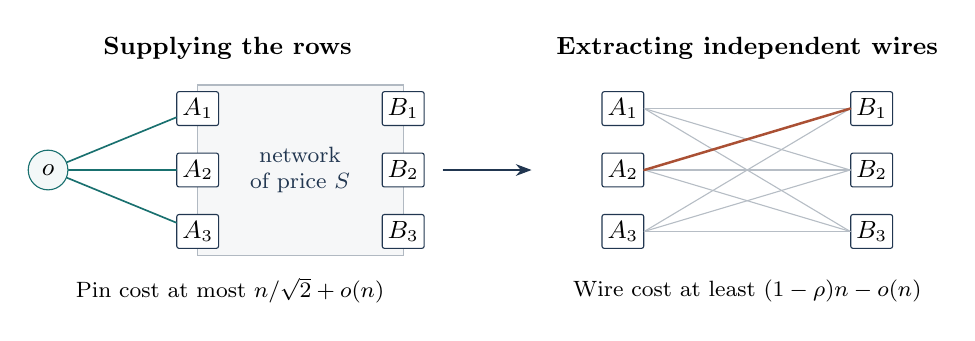
\begin{tikzpicture}[font=\small,x=1cm,y=1cm,line cap=round,
 term/.style={minimum height=.43cm,minimum width=.52cm,inner sep=2pt,
              draw=ink,fill=white,rounded corners=.8pt},
 source/.style={draw=sea,fill=sea!5,circle,inner sep=3pt}]
\begin{scope}[xshift=-3.3cm]
  \node[font=\small\bfseries] at (0,1.55){Supplying the rows};
  \filldraw[fill=ink!4,draw=ink!35] (-.38,-1.08) rectangle (2.23,1.08);
  \node[align=center,text=ink,font=\footnotesize] at (.92,0)
     {network\\of price $S$};
  \node[source] (root) at (-2.28,0) {$o$};
  \foreach \i/\y in {1/.78,2/0,3/-.78}{
    \node[term] (A\i) at (-.38,\y) {$A_\i$};
    \node[term] at (2.23,\y) {$B_\i$};
    \draw[sea,line width=.6pt] (root)--(A\i);
  }
  \node[font=\footnotesize,align=center] at (.03,-1.53)
    {Pin cost at most $n/\sqrt2+o(n)$};
\end{scope}
\draw[ink,-{Stealth[length=2mm]}] (-.56,0)--(.56,0);
\begin{scope}[xshift=3.3cm]
  \node[font=\small\bfseries] at (0,1.55){Extracting independent wires};
  \foreach \i/\y in {1/.78,2/0,3/-.78}{
     \node[term] (left\i) at (-1.58,\y) {$A_\i$};
     \node[term] (right\i) at (1.58,\y) {$B_\i$};
  }
  \foreach \i in {1,...,3}\foreach\j in {1,...,3}
    \draw[ink!33,thin] (left\i.east)--(right\j.west);
  \draw[rust,line width=.9pt] (left2.east)--(right1.west);
  \node[font=\footnotesize,align=center] at (0,-1.53)
    {Wire cost at least $(1-\rho)n-o(n)$};
\end{scope}
\end{tikzpicture}
\caption{An array bit in position $(2,1)$ appears at row terminal $A_2$
and column terminal $B_1$. Over many uses, Lemma~\ref{lem:entropy}
turns these paired copies into independent wires, with a rate for
each pair given by its conditional entropy. The prices shown are per
use, with $n=N^2$ as $N$ grows. Three rows and columns illustrate the
pairing.}
\label{fig:advice}
\end{figure}


\subsection{From adaptive heads to a network}

\begin{theorem}[Transposition on a subset of inputs]\label{thm:transpose}
Assume Weak ETH and fix $0\le\rho<1-1/\sqrt2$. On a fixed deterministic
multitape machine $\mathcal M$, suppose that by time
$T$ it has halted with the correct transpose on a fraction at least
$2^{-\rho N^2}$ of all binary $N\times N$ matrices. Inputs and outputs occupy prescribed contiguous
intervals in row-major order. The initial machine configuration may
include auxiliary data fixed independently of the matrix. Then, at
every sufficiently large side length $N$,
\[
                 T=\Omega_{\mathcal M,\rho}(N^2\sqrt{\log N}).
\]
The constants and threshold are uniform over the auxiliary data.
In particular the bound holds for the worst-case time of an exact
transposition machine.
\end{theorem}

\begin{proof}
Fix the auxiliary data and let $\mathcal G$ be the matrices correctly
transposed by time $T$. We may assume $T\le N^2\sqrt{\log N}$. Divide
each tape into blocks of $N$ consecutive cells and the first $T$ steps
into epochs of $N$ steps. Use at least one epoch, pad the final epoch,
and freeze each halted configuration while enforcing the deadline.

At each epoch boundary record just the block containing each head.
A head's recorded block number changes by at most one per epoch, so
there are at most $2^{O_{\mathcal M}(1+T/N)}$ records with the fixed
starting positions. Keep a record shared by the largest number of
inputs in $\mathcal G$. The fraction of \emph{all} matrices in this
set is at least
\[
             2^{-\rho N^2-O_{\mathcal M}(1+T/N)}.
\]
Choose any fixed $\rho'$ between $\rho$ and $1-1/\sqrt2$. Since
$T/N=O(N\sqrt{\log N})=o(N^2)$, the fraction is at least
$2^{-\rho'N^2}$ for all sufficiently large $N$. Individual head
offsets and scanned symbols can still differ on these inputs.

Build a network with one vertex per epoch, using the recorded block
numbers to specify the graph (compare the blocking method of
\cite{hpv}). During an epoch a head can meet only its starting block
and its two neighbors. For each of these blocks carry its contents
after the epoch to the next epoch in whose neighborhood it appears.
Pass the control state and each head's offset in its boundary block
to the next epoch. The contents of a block require $O_{\mathcal M}(N)$
bits and all offsets and control information require
$O_{\mathcal M}(1+\log N)$ bits.

Figure~\ref{fig:epoch-block} shows how an epoch can pass the contents of
a block directly over an intervening epoch that cannot reach it.

\begin{figure}[!htb]
\centering
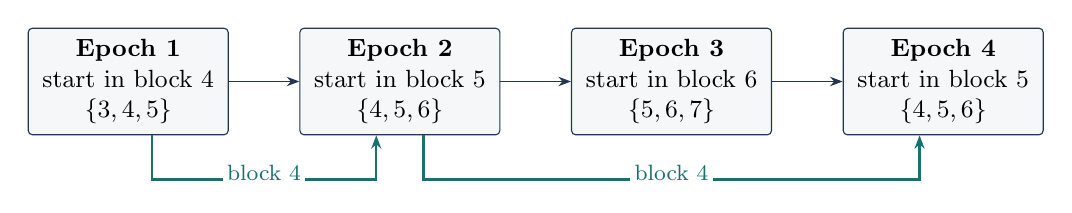
\begin{tikzpicture}[font=\small,
 epoch/.style={draw=ink,rounded corners=1.5pt,fill=ink!4,align=center,
               inner xsep=5pt,inner ysep=4pt,minimum width=2.54cm},
 state/.style={draw=ink,-{Stealth[length=1.6mm]},line width=.5pt},
 memory/.style={draw=sea,-{Stealth[length=1.7mm]},line width=.8pt}]
\foreach \i/\x/\b/\neighbors in
  {1/0/4/{3,4,5},2/3.45/5/{4,5,6},3/6.90/6/{5,6,7},4/10.35/5/{4,5,6}}{
  \node[epoch] (E\i) at (\x,0)
    {\textbf{Epoch \i}\\ start in block $\b$\\ $\{\neighbors\}$};
}
\foreach \i/\j in {1/2,2/3,3/4}
   \draw[state] (E\i.east)--(E\j.west);
\draw[memory] ([xshift=3mm]E1.south) -- ++(0,-.56)
   -| ([xshift=-3mm]E2.south);
\draw[memory] ([xshift=3mm]E2.south) -- ++(0,-.56)
   -| ([xshift=-3mm]E4.south);
\node[font=\footnotesize,text=sea,fill=white,inner sep=1.5pt] at (1.725,-1.16)
      {block $4$};
\node[font=\footnotesize,text=sea,fill=white,inner sep=1.5pt] at (6.9,-1.16)
      {block $4$};
\end{tikzpicture}
\caption{Four epochs on one tape, each labeled by the blocks it may reach.
The horizontal edges communicate the
controller state and head offset at successive boundaries. The lower
edges carry the contents of block $4$ between possible uses. A head
starting in block $6$ during Epoch 3 cannot reach block $4$ in $N$ steps,
so its contents pass directly from Epoch 2 to Epoch 4.}
\label{fig:epoch-block}
\end{figure}

The local table for an epoch is the indicator of a legal internal
run with the specified incoming and outgoing block contents, states
and head positions. Feed each block its initial contents at first use
and read its final contents at last use. Any unused block whose
initial contents affect the output can pass them through directly.
The final state must be halted by the deadline. Thus local runs
with matching boundary data concatenate to an actual machine run,
and every run that halts by the deadline with this record satisfies the
local relations. By
determinism, on each selected input the network has support only at
the correct output, with positive coefficient.

The fixed tape count bounds the number of incident bundles per epoch.
Use a distinct terminal for each row and column. An external string
crossing a block boundary is joined from at most two consecutive
blocks, and a block meets at most two such strings at either interface.
These extra vertices preserve bounded degree. In total there are
$O_{\mathcal M}(N+1+T/N)$ vertices, with all widths
$O_{\mathcal M}(N)$. Applying Theorem~\ref{thm:table} at density
$2^{-\rho'N^2}$ gives
\[
             N+1+T/N=\Omega_{\mathcal M,\rho}(N\sqrt{\log N}),
\]
as required.
\end{proof}

\begin{proof}[Proof of the multiplication lower bound in Theorem~\ref{thm:lower}]
Let $M(m)$ be the worst-case time of a fixed exact multiplier on two
$m$-bit operands. Given $m$, the reduction of Harvey and van der Hoeven
\cite[full version, Corollaries~6.2 and~6.3]{hvhtranspose} transposes
a bit matrix of side $N=\lfloor\sqrt m\rfloor$ in
\[
                O\bigl(M(m)+m(1+\log\log(2m))\bigr)
\]
steps. In that reduction, padding to a larger dyadic length is followed
by splitting each padded multiplication into a bounded number of calls
at length $m$. Thus the bound uses the actual value $M(m)$ at the
specified length. Copying, padding and adapting the ordinary binary
input and output conventions here take $O(m)$ additional steps.

Use $m$ as auxiliary data in Theorem~\ref{thm:transpose}, with
$\rho=0$. The lower bound on the resulting transposer is uniform in
$m$. Since $N^2\sqrt{\log N}=\Theta(m\sqrt{\log m})$ and
$m(1+\log\log(2m))=o(m\sqrt{\log m})$, it follows that
$M(m)=\Omega(m\sqrt{\log m})$ at every sufficiently large $m$.
\end{proof}


\bibliographystyle{plainnat}
\bookmarksetup{startatroot}
\bibliography{references}
\end{document}
